\documentclass[aspectratio=169,10pt]{beamer}

% 使用简洁现代的主题
\usetheme{metropolis}
\usecolortheme{seahorse}

% 中文支持
\usepackage[UTF8]{ctex}
\usepackage{amsmath,amssymb,amsfonts}
\usepackage{graphicx}
\usepackage{booktabs}
\usepackage{hyperref}
\usepackage{xcolor}
\usepackage{tikz}
\usetikzlibrary{positioning,arrows.meta,shadows,shapes.geometric}
\usepackage{pgfplots}
\usepackage{multicol}
\usepackage{caption}
\usepackage{multirow}
\usepackage{colortbl}

% 设置 pgfplots 兼容
\pgfplotsset{compat=1.18}

% ============================================================
% 现代学术风格配色 - 专业、清晰、舒适
% ============================================================
% 主色调：深青蓝色（专业、稳重）
\definecolor{primaryblue}{RGB}{15,65,110}        % 深蓝 - 主标题、重点
\definecolor{secondaryblue}{RGB}{41,121,255}     % 亮蓝 - 次要元素、链接
\definecolor{lightblue}{RGB}{230,240,250}        % 浅蓝 - 背景点缀

% 强调色：珊瑚红（醒目但不刺眼）
\definecolor{accentred}{RGB}{220,53,69}          % 红色 - 警告、重点强调
\definecolor{accentorange}{RGB}{253,126,20}      % 橙色 - 次级强调

% 辅助色：青绿色（清新、积极）
\definecolor{accentgreen}{RGB}{20,160,133}       % 青绿 - 成功、正面
\definecolor{teal}{RGB}{0,150,136}               % 深青 - 数据可视化

% 中性色
\definecolor{darkgray}{RGB}{51,51,51}            % 深灰 - 正文
\definecolor{mediumgray}{RGB}{108,117,125}       % 中灰 - 次要文字
\definecolor{lightgray}{RGB}{248,249,250}        % 浅灰 - 背景
\definecolor{bordergray}{RGB}{222,226,230}       % 边框灰

% metropolis 主题颜色覆盖
\definecolor{metropolisbackground}{RGB}{255,255,255}
\definecolor{metropolisforeground}{RGB}{51,51,51}
\definecolor{metropolisblockbackground}{RGB}{248,249,250}

% 设置主题颜色
\setbeamercolor{palette primary}{bg=primaryblue,fg=white}
\setbeamercolor{palette secondary}{bg=secondaryblue,fg=white}
\setbeamercolor{palette tertiary}{bg=accentgreen,fg=white}
\setbeamercolor{palette quaternary}{bg=accentred,fg=white}
\setbeamercolor{titlelike}{bg=primaryblue,fg=white}
\setbeamercolor{frametitle}{bg=white,fg=primaryblue}
\setbeamercolor{background canvas}{bg=white}
\setbeamercolor{normal text}{fg=darkgray}
\setbeamercolor{section in toc}{fg=primaryblue,bg=white}
\setbeamercolor{section in head/foot}{fg=white,bg=primaryblue}
\setbeamercolor{title}{fg=white,bg=primaryblue}
\setbeamercolor{subtitle}{fg=white,bg=primaryblue}
\setbeamercolor{author}{fg=darkgray,bg=white}
\setbeamercolor{institute}{fg=mediumgray,bg=white}
\setbeamercolor{date}{fg=mediumgray,bg=white}

% 自定义块样式 - 现代化设计
\setbeamercolor{block title}{bg=primaryblue,fg=white}
\setbeamercolor{block body}{bg=lightblue,fg=darkgray}
\setbeamercolor{block title alerted}{bg=accentred,fg=white}
\setbeamercolor{block body alerted}{bg=lightgray,fg=darkgray}
\setbeamercolor{block title example}{bg=accentgreen,fg=white}
\setbeamercolor{block body example}{bg=lightgray,fg=darkgray}

% 表格颜色
\setbeamercolor{row 1}{bg=primaryblue,fg=white}
\setbeamercolor{row 2}{bg=lightgray,fg=darkgray}

% 超链接设置
\hypersetup{
    colorlinks=true,
    linkcolor=secondaryblue,
    filecolor=accentred,
    urlcolor=secondaryblue,
    citecolor=primaryblue,
}

% 标题页背景设计
\makeatletter
\setbeamertemplate{title page}{
    \begin{beamercolorbox}[wd=\paperwidth,ht=0.4\paperheight,center]{palette primary}
        \vfill
        {\usebeamerfont{title}\usebeamercolor[fg]{title}\Huge\bfseries\inserttitle\par}
        \vspace{1em}
        {\usebeamerfont{subtitle}\usebeamercolor[fg]{subtitle}\Large\insertsubtitle\par}
        \vfill
    \end{beamercolorbox}
    \vfill
    {\usebeamerfont{author}\usebeamercolor[fg]{author}\large\insertauthor\par}
    \vspace{0.5em}
    {\usebeamerfont{institute}\usebeamercolor[fg]{institute}\small\insertinstitute\par}
    \vspace{0.5em}
    {\usebeamerfont{date}\usebeamercolor[fg]{date}\small\insertdate\par}
    \vfill
}

% 章节页样式 - 渐变背景
\AtBeginSection{
    \begin{frame}
        \vfill
        \centering
        
\begin{tikzpicture}[remember picture,overlay]
            \fill[top color=primaryblue,bottom color=secondaryblue]
                (current page.south west) rectangle (current page.north east);
        \end{tikzpicture}
        \begin{beamercolorbox}[sep=12pt,center,rounded=true,shadow=true]{title}
            \usebeamerfont{title}\Large\color{white}\bfseries\insertsectionhead\par
        \end{beamercolorbox}
        \vfill
    \end{frame}
}

% 页脚设计
\setbeamertemplate{footline}{
    \begin{beamercolorbox}[wd=\paperwidth,ht=0.6cm,dp=0.3cm]{palette primary}
        \hspace*{1em}\tiny\insertshortauthor\hfill
        \tiny\insertshorttitle
        \hfill \tiny\insertframenumber{} / \inserttotalframenumber\hspace*{1em}
    \end{beamercolorbox}
}

% ============================================================
% 字体优化 - 更清晰、更现代
% ============================================================
% 设置页面布局
\raggedbottom
\setlength{\belowcaptionskip}{0.5em}

% 设置正文字体
\setbeamerfont{normal text}{size=\footnotesize,series=\mdseries}
\setbeamerfont{title}{size=\Large,series=\bfseries}
\setbeamerfont{frametitle}{size=\large,series=\bfseries}
\setbeamerfont{block title}{size=\small,series=\bfseries}
\setbeamerfont{block body}{size=\footnotesize}
\setbeamerfont{itemize/enumerate}{size=\footnotesize}

% 标题页字体
\setbeamerfont{title}{size=\large,series=\bfseries}
\setbeamerfont{subtitle}{size=\normalsize,series=\mdseries}
\setbeamerfont{author}{size=\small,series=\mdseries}
\setbeamerfont{institute}{size=\footnotesize,series=\mdseries}
\setbeamerfont{date}{size=\footnotesize,series=\mdseries}

% 标题信息
\title{基于表格型 Q-Learning 的运动想象脑电信号时间窗优化方法研究}
\subtitle{毕业设计中期考核报告}
\author{邓凯璇}
\institute{
    姓名：邓凯璇 \quad|\quad 学号：37220222203575 \\
    学院：信息学院 \quad|\quad 专业：人工智能 \\
    指导教师：施明辉
}
\date{\today}

\begin{document}
 
% 标题页
\begin{frame}
    \titlepage
\end{frame}

% 目录页
\begin{frame}{报告提纲}
    \vspace{1em}
    \tableofcontents
\end{frame}

% 导入章节
% 第一部分：引言
\section{引言}

\begin{frame}{研究背景}
    \begin{block}{\normalsize 运动想象脑机接口}
        \begin{itemize}
            \item[\textcolor{primaryblue}{\textbullet}] \textbf{核心任务}：通过分类脑电信号（EEG）中的事件相关去同步化（ERD）模式，识别用户的运动想象意图
            \item[\textcolor{primaryblue}{\textbullet}] \textbf{关键挑战}：EEG 信号的非平稳性和个体差异性导致时间窗选择成为影响分类性能的关键因素
        \end{itemize}
    \end{block}

    \vspace{0.5em}

    \begin{alertblock}{\normalsize 现有时间窗选择策略的局限}
        \begin{itemize}
            \item[\textcolor{accentred}{\textbullet}] \textbf{固定时间窗方法}：依赖先验知识选择固定时间段，难以适应个体差异
            \item[\textcolor{accentred}{\textbullet}] \textbf{深度强化学习方法（DQN）}：通过神经网络近似 Q 函数实现自适应优化，但存在模型复杂度高、训练不稳定、可解释性差等问题
        \end{itemize}
    \end{alertblock}
\end{frame}

\begin{frame}{研究问题与核心主张}
    \begin{block}{\normalsize 研究问题}
        如何在运动想象时间窗优化任务中，在保持与 DQN 相当性能的同时，显著降低模型复杂度、提升系统稳定性和可解释性？
    \end{block}

    \vspace{0.5em}

    \begin{exampleblock}{\normalsize 核心主张}
        在运动想象时间窗优化这一特定任务中，\textbf{表格型 Q-Learning} 可以在保持与 DQN 相当性能的同时，显著降低模型复杂度，提升系统稳定性和可解释性，更适合在资源受限的嵌入式 BCI 设备中部署。
    \end{exampleblock}
\end{frame}

\begin{frame}{轻量化设计动机}
    \begin{columns}[T]
        \begin{column}{0.31\textwidth}
            \begin{block}{\centering \normalsize 动机一：数据约束}
                \begin{itemize}
                    \item \textbf{数据稀缺性}：EEG 数据采集成本高，伦理审查严格
                    \item \textbf{个体差异性}：跨被试泛化困难，需快速独立训练
                    \item \textbf{样本效率}：有限样本下快速收敛
                \end{itemize}
            \end{block}
        \end{column}

        \begin{column}{0.31\textwidth}
            \begin{block}{\centering \normalsize 动机二：设备约束}
                \begin{itemize}
                    \item \textbf{硬件成本}：ARM Cortex-M 等低功耗嵌入式处理器
                    \item \textbf{能耗约束}：电池供电，需最小化计算能耗
                    \item \textbf{实时性}：毫秒级延迟完成时间窗选择
                \end{itemize}
            \end{block}
        \end{column}

        \begin{column}{0.31\textwidth}
            \begin{block}{\centering \normalsize 动机三：任务定位}
                \begin{itemize}
                    \item \textbf{辅助任务从属性}：时间窗选择服务于分类任务
                    \item \textbf{计算预算分配}：资源优先分配给核心任务
                    \item \textbf{性能 - 效率权衡}：遵循"足够好"原则
                \end{itemize}
            \end{block}
        \end{column}
    \end{columns}

    \vspace{0.5em}

    \begin{exampleblock}{\normalsize 设计原则}
        \centering 时间窗优化算法应在保证性能的前提下，最大化轻量化和高效性，以适应 BCI 技术的数据约束、部署约束和任务定位约束
    \end{exampleblock}
\end{frame}

\begin{frame}{研究意义}
    \begin{columns}[T]
        \begin{column}{0.48\textwidth}
            \begin{block}{\normalsize \textcolor{primaryblue}{理论意义}}
                \begin{itemize}
                    \item \textbf{挑战深度强化学习的"必要性"假设}：证明简单方法在特定场景下可能是更优选择
                    \item \textbf{提出 BCI 轻量化设计框架}：系统阐述轻量化设计的三方面动机和实现路径
                    \item \textbf{界定表格型与深度方法的适用边界}：状态空间规模 $< 10^4$ 时表格型方法更优
                \end{itemize}
            \end{block}
        \end{column}

        \begin{column}{0.48\textwidth}
            \begin{block}{\normalsize \textcolor{accentgreen}{实际意义}}
                \begin{itemize}
                    \item \textbf{适合嵌入式 BCI 设备}：内存占用 KB 级，无需深度学习框架
                    \item \textbf{降低部署成本}：可移植至 ARM Cortex-M 等平台
                    \item \textbf{提升系统响应性}：推理延迟降低 1000 倍，改善用户体验
                \end{itemize}
            \end{block}
        \end{column}
    \end{columns}
\end{frame}

% 第二部分：引言与相关工作
\section{引言与相关工作}

\begin{frame}{研究背景与意义}
    \begin{block}{\normalsize 脑机接口技术}
        \begin{itemize}
            \item[\textcolor{primaryblue}{\textbullet}] \textbf{BCI 技术}：直接连接大脑与外部设备的新型交互技术
            \item[\textcolor{primaryblue}{\textbullet}] \textbf{应用领域}：医疗康复、神经工程、智能控制
            \item[\textcolor{primaryblue}{\textbullet}] \textbf{运动想象范式}：通过解码 ERD/ERS 脑电信号实现无外部刺激下的自然控制
        \end{itemize}
    \end{block}

    \vspace{0.3em}

    \begin{alertblock}{\normalsize 关键挑战：时间窗选择问题}
        \begin{itemize}
            \item[\textcolor{accentred}{\textbullet}] \textbf{固定时间窗局限}：忽视神经响应的个体差异性和任务依赖性
            \item[\textcolor{accentred}{\textbullet}] \textbf{个体差异显著}：不同被试的 ERD/ERS 起始时间和持续时间存在明显差异
            \item[\textcolor{accentred}{\textbullet}] \textbf{性能影响}：固定时间窗导致信号信息丢失或噪声引入，降低分类性能
        \end{itemize}
    \end{alertblock}

    \vspace{0.3em}

    \begin{exampleblock}{\normalsize 研究意义}
        开发能够\textbf{自适应调整时间窗参数}的智能方法，对于提升 MI-BCI 系统的实用性和鲁棒性具有重要意义
    \end{exampleblock}
\end{frame}

\begin{frame}{传统时间窗优化方法}
    \begin{columns}[T]
        \begin{column}{0.48\textwidth}
            \begin{block}{\normalsize 早期方法}
                \begin{itemize}
                    \item \textbf{经验法}：依靠经验或试错法确定时间窗口
                    \item \textbf{固定时间窗}：采用统一时间段（如 2-4 秒）
                    \item \textbf{手动选择}：基于先验知识人工设定
                \end{itemize}
            \end{block}
        \end{column}

        \begin{column}{0.48\textwidth}
            \begin{alertblock}{\normalsize 自动化优化方法}
                \begin{itemize}
                    \item \textbf{网格搜索与随机搜索}
                    \begin{itemize}
                        \item 遍历或随机采样参数空间
                        \item 计算成本随维度指数增长
                        \item 缺乏理论指导
                    \end{itemize}

                    \item \textbf{贝叶斯优化}
                    \begin{itemize}
                        \item Yang 等：双独立贝叶斯优化框架
                        \item 代理模型训练复杂
                        \item 缺乏时间窗参数内在关联性建模
                    \end{itemize}

                    \item \textbf{启发式算法}
                    \begin{itemize}
                        \item 蚁群优化、遗传算法等
                        \item 易陷入局部最优
                        \item 收敛性难以保证
                    \end{itemize}
                \end{itemize}
            \end{alertblock}
        \end{column}
    \end{columns}
\end{frame}

\begin{frame}{强化学习在 BCI 中的应用}
    \begin{block}{\normalsize 主要应用方向}
        \begin{itemize}
            \item[\textcolor{primaryblue}{\textbullet}] \textbf{动态窗口控制}
            \begin{itemize}
                \item Chen 等 (2019)：DQN 用于 SSVEP 识别，动态调整采集窗口长度
                \item 针对 SSVEP 范式设计，不直接适用于 MI 任务
            \end{itemize}

            \vspace{0.5em}
            \item[\textcolor{primaryblue}{\textbullet}] \textbf{特征选择优化}
            \begin{itemize}
                \item Zhang 等 (2021)：多智能体 RL 框架 MARS
                \item 用于空间 - 频域和时域特征选择
                \item 主要关注特征层面而非原始信号时间窗截取
            \end{itemize}

            \vspace{0.5em}
            \item[\textcolor{primaryblue}{\textbullet}] \textbf{参数自适应调整}
            \begin{itemize}
                \item 优化 BCI 系统参数（分类器超参数、滤波器设置）
                \item 专门针对时间窗优化的研究仍属空白
            \end{itemize}
        \end{itemize}
    \end{block}
\end{frame}

\begin{frame}{强化学习算法演进}
    \begin{columns}[T]
        \begin{column}{0.58\textwidth}
            \begin{block}{\normalsize 经典算法}
                \begin{itemize}
                    \item \textbf{Q-learning}
                    \begin{itemize}
                        \item 经典表格型 RL 算法
                        \item 在离散状态空间中表现稳定
                        \item 存在 Q 值过高估计问题
                    \end{itemize}
                \end{itemize}
            \end{block}


            \begin{alertblock}{\normalsize 增强算法}
                \begin{itemize}
                    \item \textbf{Double Q-learning}：维护两套独立的 Q 值估计交替用于动作选择和值评估缓解 Q 值过高估计问题
                    \item \textbf{Dueling Network 架构}：分解为状态价值函数和动作优势函数分别评估状态好坏和动作相对优势提升学习效率和策略质量
                \end{itemize}
            \end{alertblock}
        \end{column}

        \begin{column}{0.48\textwidth}
            \begin{exampleblock}{\normalsize 深度 Q 网络变体}
                \begin{itemize}
                    \item 结合深度神经网络的函数逼近能力
                    \item 需要大量数据和复杂调参
                    \item 在有限状态空间问题中可能过度复杂
                \end{itemize}

                \vspace{0.5em}

                \begin{itemize}
                    \item \textbf{技术演进路线}：
                    \begin{enumerate}
                        \item 表格型 RL (1990s)
                        \item 值函数近似 (2000s)
                        \item 深度 RL (2015-)
                        \item \textcolor{primaryblue}{\textbf{轻量化 RL (本研究)}}
                    \end{enumerate}
                \end{itemize}
            \end{exampleblock}
        \end{column}
    \end{columns}
\end{frame}

\begin{frame}{现有研究不足}
    \begin{alertblock}{\normalsize 研究空白}
        \begin{itemize}
            \item[\textcolor{accentred}{\textbullet}] \textbf{方法适用性局限}
            \begin{itemize}
                \item 现有时间窗优化方法多基于传统优化理论
                \item 未充分利用 RL 的序列决策和自适应学习优势
            \end{itemize}

            \vspace{0.5em}
            \item[\textcolor{accentred}{\textbullet}] \textbf{个体差异考虑不足}
            \begin{itemize}
                \item 大多数方法采用统一优化策略
                \item 缺乏对神经响应个体差异性的专门建模
            \end{itemize}

            \vspace{0.5em}
            \item[\textcolor{accentred}{\textbullet}] \textbf{算法复杂度失衡}
            \begin{itemize}
                \item 简单方法性能有限
                \item 先进方法（如深度 RL）实现复杂且需要大量计算资源
            \end{itemize}
        \end{itemize}
    \end{alertblock}
\end{frame}

\begin{frame}{本工作创新点}
    \begin{exampleblock}{\normalsize 创新性工作}
        \begin{itemize}
            \item[\textcolor{primaryblue}{\textbullet}] \textbf{设计面向时间窗优化的 RL 机制}
            \begin{itemize}
                \item 将连续时间参数离散化为适合 RL 处理的形式
                \item 保持生理合理性约束
                \item 设计状态 - 动作 - 奖励机制
            \end{itemize}

            \vspace{0.5em}
            \item[\textcolor{primaryblue}{\textbullet}] \textbf{提出计算高效的表格型实现方案}
            \begin{itemize}
                \item 针对有限状态空间特点
                \item 避免不必要的深度网络复杂度
                \item 确保方法在标准计算设备上的可行性
            \end{itemize}

            \vspace{0.5em}
            \item[\textcolor{primaryblue}{\textbullet}] \textbf{构建端到端的个性化优化框架}
            \begin{itemize}
                \item 为每个被试独立学习最优时间窗参数
                \item 显著提升 MI 分类性能
            \end{itemize}
        \end{itemize}
    \end{exampleblock}
\end{frame}

% 第三部分：方法
\section{方法}

\begin{frame}{方法整体框架}
    \begin{block}{\normalsize 两阶段处理流程}
        \centering
        \begin{tikzpicture}[
            node distance=0.8cm,
            phase/.style={rectangle, draw=primaryblue, fill=lightblue,
                         rounded corners=4pt, inner sep=8pt, font=\footnotesize\bfseries},
            box/.style={rectangle, draw=darkgray, fill=white,
                       rounded corners=4pt, inner sep=6pt, font=\footnotesize},
            arrow/.style={->, >=Stealth, thick, primaryblue},
            data/.style={trapezium, trapezium left angle=70, trapezium right angle=110,
                        draw=accentgreen, fill=green!10, inner sep=4pt, font=\footnotesize}
        ]
            % 训练阶段
            \node[phase, fill=primaryblue!15] (trainphase) {
                \begin{tabular}{c}
                    \textcolor{primaryblue}{\Large\textbullet} 训练阶段
                \end{tabular}
            };
            
            \node[box, above=0.3cm of trainphase] (preprocess) {
                \begin{tabular}{c}
                    数据预处理 \\
                    \scriptsize 带通滤波、陷波滤波、平均参考
                \end{tabular}
            };
            
            \node[box, below=0.3cm of trainphase] (qlearn) {
                \begin{tabular}{c}
                    Q-Learning 训练 \\
                    \scriptsize $\epsilon$-贪婪策略、Q 值更新
                \end{tabular}
            };
            
            \node[data, left=0.5cm of trainphase] (eegdata) {EEG 数据};
            
            \draw[arrow] (eegdata) -- (trainphase);
            \draw[arrow] (preprocess) -- (trainphase);
            \draw[arrow] (trainphase) -- (qlearn);
            
            % 测试阶段
            \node[phase, right=3cm of trainphase, fill=secondaryblue!15] (testphase) {
                \begin{tabular}{c}
                    \textcolor{secondaryblue}{\Large\textbullet} 测试阶段
                \end{tabular}
            };
            
            \node[box, above=0.3cm of testphase] (csp) {
                \begin{tabular}{c}
                    CSP 特征提取 \\
                    \scriptsize 空间滤波、对数方差
                \end{tabular}
            };
            
            \node[box, below=0.3cm of testphase] (svm) {
                \begin{tabular}{c}
                    SVM 分类 \\
                    \scriptsize 线性核、类别预测
                \end{tabular}
            };
            
            \node[data, right=0.5cm of testphase] (output) {分类结果};
            
            \draw[arrow] (testphase) -- (csp);
            \draw[arrow] (testphase) -- (svm);
            \draw[arrow] (testphase) -- (output);
            
            % 阶段连接
            \draw[arrow, dashed] (qlearn.east) -- node[above, font=\tiny] {Q 值表} (testphase.west);
        \end{tikzpicture}
    \end{block}


\end{frame}

\begin{frame}{MDP 问题形式化}
    \begin{block}{\normalsize 马尔可夫决策过程五元组 $(\mathcal{S}, \mathcal{A}, \mathcal{R}, \mathcal{P}, \gamma)$}
        \vspace{0.3em}
        \centering
        \begin{tikzpicture}[
            node distance=0.4cm,
            comp/.style={rectangle, rounded corners=4pt, 
                        inner sep=4pt, font=\small, minimum width=5cm, align=center}
        ]
            \node[comp, draw=primaryblue, fill=primaryblue!15, align=left] (state) {
                \textbf{\color{primaryblue}状态空间 $\mathcal{S}$} \\
                \scriptsize 离散化时间窗参数 $s = (t_{\text{start}}, t_{\text{end}})$ \\
                \scriptsize $t_{\text{start}} \in [0.0, 3.0]$s, 步长 0.2s \\
                \scriptsize $t_{\text{end}} \in [1.0, 4.0]$s, 步长 0.2s \\
                \scriptsize 约束：$t_{\text{end}} - t_{\text{start}} \geq 0.5$s \\
                \scriptsize \textbf{\color{accentgreen}有效状态数：$|\mathcal{S}| = 136$}
            };
            
            \node[comp, draw=secondaryblue, fill=secondaryblue!15, right=0.2cm of state, align=left] (action) {
                \textbf{\color{secondaryblue}动作空间 $\mathcal{A}$} \\
                \scriptsize 4 个离散动作 $\mathcal{A} = \{a_0, a_1, a_2, a_3\}$ \\
                \scriptsize $a_0$: $t_{\text{start}} \!-\! 0.2$s \quad $a_1$: $t_{\text{start}} \!+\! 0.2$s \\
                \scriptsize $a_2$: $t_{\text{end}} \!-\! 0.2$s \quad $a_3$: $t_{\text{end}} \!+\! 0.2$s \\
                \scriptsize \textbf{Q 表大小：$136 \times 4 = 544$}
            };
            
            \node[comp, draw=accentred, fill=accentred!15, below=of state, align=left] (reward) {
                \textbf{\color{accentred}奖励函数 $\mathcal{R}$} \\
                \scriptsize $\mathcal{R}(s) = \text{Accuracy}_{\text{CV}}(t_{\text{start}}, t_{\text{end}})$ \\
                \scriptsize 当前时间窗下 CSP-SVM 的 \\
                \scriptsize 5 折交叉验证准确率
            };
            
            \node[comp, draw=accentgreen, fill=accentgreen!15, below=of action, align=left] (transition) {
                \textbf{\color{accentgreen}状态转移 $\mathcal{P}$} \\
                \scriptsize 确定性转移：动作执行后 \\
                \scriptsize 时间窗边界按固定步长调整 \\
                \scriptsize 超出范围则保持原状态
            };
            
            \node[comp, draw=darkgray, fill=gray!15, below=of reward, xshift=5.1cm, minimum width=10.2cm] (gamma) {
                \textbf{折扣因子 $\gamma = 0.95$} \quad 
                \scriptsize 平衡即时奖励与长期奖励
            };
        \end{tikzpicture}
    \end{block}
\end{frame}


\begin{frame}{表格型 Q-Learning 算法}
    \begin{columns}[T]
        \begin{column}{0.55\textwidth}
            \begin{block}{\normalsize Q 值更新规则}
                \footnotesize
                遵循 Bellman 最优方程：
                $$Q(s_t, a_t) \leftarrow Q(s_t, a_t) + \alpha \left[ r_{t+1} + \gamma \max_{a} Q(s_{t+1}, a) - Q(s_t, a_t) \right]$$
                
            \end{block}


            \begin{block}{\normalsize 收敛性保证}
                \footnotesize
                \textbf{定理}（Watkins \& Dayan, 1992）：对于有限 MDP，若满足：
                \begin{enumerate}
                    \item 所有状态 - 动作对被无限次访问
                    \item 学习率满足 Robbins-Monro 条件
                    \item 采用适当的探索策略（如$\epsilon$-贪婪）
                \end{enumerate}
                则 Q 值序列以概率 1 收敛到最优动作价值函数 $Q^*$。
            \end{block}
        \end{column}

        \begin{column}{0.5\textwidth}

            \begin{block}{\normalsize 本研究适用性}
                \footnotesize
                \begin{itemize}
                    \item 状态空间有限（136 个状态）、动作空间有限（4 个动作）
                    \item $\epsilon$-贪婪策略保证充分探索
                    \item \textbf{理论保证收敛到最优策略}
                \end{itemize}
            \end{block}
        \end{column}
    \end{columns}
\end{frame}

\begin{frame}{Q-Learning 算法流程}
    \centering
    \resizebox{0.95\textwidth}{!}{
    \begin{tikzpicture}[
        node distance=0.5cm and 0.6cm,
        startstop/.style={rectangle, rounded corners, draw=accentred, fill=red!10,
                         text width=4.5em, text centered, minimum height=1.3em, font=\small},
        process/.style={rectangle, draw=primaryblue, fill=lightblue,
                       text width=5.5em, text centered, minimum height=1.3em, font=\small},
        decision/.style={diamond, draw=secondaryblue, fill=blue!10,
                        text width=4em, text centered, minimum height=1.3em, font=\small, aspect=1.2},
        arrow/.style={->, >=Stealth, thick, darkgray},
        io/.style={trapezium, trapezium left angle=70, trapezium right angle=110,
                  draw=accentgreen, fill=green!10, text width=4.5em, text centered,
                  minimum height=1.3em, font=\small}
    ]
        % 主流程（水平方向）
        \node[io] (init) {初始化 Q 表\\$\epsilon=0.9$};
        \node[process, right=of init] (eploop) {Episode 循环\\(1-100)};
        \node[process, right=of eploop] (initstate) {随机初始化\\状态 $s_0$};
        \node[process, right=of initstate] (steploop) {Step 循环\\(1-40)};
        \node[decision, right=of steploop] (epsdecision) {$\text{random}<\epsilon$?};
        
        % 分支节点（上下布局）
        \node[process, above=0.8cm of epsdecision] (explore) {随机探索\\动作};
        \node[process, below=0.8cm of epsdecision] (exploit) {贪婪选择\\$\arg\max Q$};
        
        % 后续流程（水平方向）
        \node[process, right=1.2cm of epsdecision] (execute) {执行动作\\状态转移};
        \node[process, right=of execute] (evaluate) {Evaluate};
        \node[process, right=of evaluate] (updateq) {更新 Q 值};
        \node[process, right=of updateq] (decayeps) {$\epsilon$ 衰减\\$\times 0.995$};
        \node[startstop, right=of decayeps] (output) {输出最优\\时间窗};

        % 箭头连接
        \draw[arrow] (init) -- (eploop);
        \draw[arrow] (eploop) -- (initstate);
        \draw[arrow] (initstate) -- (steploop);
        \draw[arrow] (steploop) -- (epsdecision);
        \draw[arrow] (epsdecision) -- node[left, font=\tiny] {是} (explore);
        \draw[arrow] (epsdecision) -- node[right, font=\tiny] {否} (exploit);
        \draw[arrow] (explore) -| (execute);
        \draw[arrow] (exploit) -| (execute);
        \draw[arrow] (execute) -- (evaluate);
        \draw[arrow] (evaluate) -- (updateq);
        \draw[arrow] (updateq) -- (decayeps);
        \draw[arrow] (decayeps) -- (output);

        % 循环反馈
        \draw[arrow, rounded corners] (output.north) -- ++(0,0.8) -| node[pos=0.25, above, font=\tiny] {step<40} (steploop.north);
        \draw[arrow, rounded corners] (output.south) -- ++(0,-0.8) -| node[pos=0.25, below, font=\tiny] {episode<100} (eploop.south);
    \end{tikzpicture}
    }

    \vspace{0.3em}

    \begin{alertblock}{\normalsize 关键设计}
        \footnotesize
        \begin{itemize}
            \item \textbf{$\epsilon$-贪婪策略}：训练初期充分探索（$\epsilon=0.9$），后期逐渐利用（$\epsilon_{\min}=0.05$）
            \item \textbf{随机初始化}：确保训练初期状态空间覆盖
            \item \textbf{早停机制}：Q 值收敛或最优状态稳定时提前终止
        \end{itemize}
    \end{alertblock}
\end{frame}

\begin{frame}{时间窗评估子过程}
    \centering
    \resizebox{0.92\textwidth}{!}{
    \begin{tikzpicture}[
        node distance=0.4cm and 0.5cm,
        startstop/.style={rectangle, rounded corners, draw=accentred, fill=red!10,
                         text width=4.5em, text centered, minimum height=1.3em, font=\small},
        process/.style={rectangle, draw=primaryblue, fill=lightblue,
                       text width=5.5em, text centered, minimum height=1.3em, font=\small},
        arrow/.style={->, >=Stealth, thick, darkgray},
        io/.style={trapezium, trapezium left angle=70, trapezium right angle=110,
                  draw=accentgreen, fill=green!10, text width=4.5em, text centered,
                  minimum height=1.3em, font=\small}
    ]
        % 主流程（水平方向）
        \node[io] (input) {输入状态 $s$\\训练数据};
        \node[process, right=of input] (window) {时间窗截取\\$X_i^{\text{window}}$};
        \node[process, right=of window] (cov) {计算协方差\\矩阵 $C_c$};
        \node[process, right=of cov] (eigen) {广义特征值\\分解};
        \node[process, right=of eigen] (filter) {构建空间\\滤波器 $W$};
        \node[process, right=of filter] (feature) {提取对数\\方差特征};
        \node[process, right=of feature] (normalize) {Z-score\\标准化};
        \node[process, right=of normalize] (cv) {5 折交叉\\验证 SVM};
        \node[io, right=of cv] (output) {返回平均\\准确率};

        % 箭头连接
        \draw[arrow] (input) -- (window);
        \draw[arrow] (window) -- (cov);
        \draw[arrow] (cov) -- (eigen);
        \draw[arrow] (eigen) -- (filter);
        \draw[arrow] (filter) -- (feature);
        \draw[arrow] (feature) -- (normalize);
        \draw[arrow] (normalize) -- (cv);
        \draw[arrow] (cv) -- (output);
    \end{tikzpicture}
    }

    \vspace{0.3em}

    \begin{columns}[T]
        \begin{column}{0.48\textwidth}
            \begin{alertblock}{\normalsize CSP 核心思想}
                \footnotesize
                通过空间滤波最大化两类信号的方差差异：
                $$C_1 \cdot w = \lambda \cdot (C_1 + C_2) \cdot w$$
            \end{alertblock}
        \end{column}

        \begin{column}{0.48\textwidth}
            \begin{exampleblock}{\normalsize SVM 分类器}
                \footnotesize
                线性核，$C = 1.0$，5 折交叉验证：
                $$\min_{w,b} \frac{1}{2}||w||^2 + C \cdot \sum \xi_i$$
            \end{exampleblock}
        \end{column}
    \end{columns}
\end{frame}

\begin{frame}{与 DQN 的对比分析}
    \begin{columns}[t]
        \begin{column}{0.52\textwidth}
            \begin{table}
                \centering
                \footnotesize
                \begin{tabular}{lcc}
                    \toprule
                    \textbf{维度} & \textbf{表格型 Q} & \textbf{DQN} \\
                    \midrule
                    函数近似 & 无（精确表） & 深度神经网络 \\
                    \rowcolor{lightblue}
                    参数量 & \textasciitilde544 & \textasciitilde10⁴–10⁵ \\
                    收敛性保证 & \textcolor{accentgreen}{理论保证} & 经验性收敛 \\
                    \rowcolor{lightblue}
                    训练稳定性 & \textcolor{accentgreen}{高} & 中 \\
                    推理延迟 & \textcolor{accentgreen}{\textasciitilde0.1 μs} & \textasciitilde100 μs \\
                    \rowcolor{lightblue}
                    内存占用 & \textcolor{accentgreen}{\textasciitilde2 KB} & \textasciitilde100 KB–1 MB \\
                    可解释性 & \textcolor{accentgreen}{高} & 低 \\
                    \rowcolor{lightblue}
                    泛化能力 & 中 & \textcolor{accentgreen}{高} \\
                    适用场景 & \textcolor{accentgreen}{小规模状态空间} & 大规模状态空间 \\
                    \bottomrule
                \end{tabular}
            \end{table}
        \end{column}

        \begin{column}{0.46\textwidth}
            \vspace{-0.5em}
            \begin{alertblock}{\normalsize DQN 方法回顾}
                \scriptsize
                DQN 使用深度神经网络近似 Q 函数：
                \[Q(s, a; \theta) \approx Q^*(s, a)\]
                损失函数：
                \[\mathcal{L}(\theta) = \mathbb{E}\left[ \left( r + \gamma \max_{a'} Q(s', a'; \theta^-) - Q(s, a; \theta) \right)^2 \right]\]
            \end{alertblock}

            \begin{exampleblock}{\normalsize 本研究核心主张}
                \scriptsize
                \begin{itemize}
                    \item \textbf{主张 1}：与 DQN 准确率无显著差异
                    \item \textbf{主张 2}：跨被试标准差更低
                    \item \textbf{主张 3}：更适合嵌入式部署
                    \item \textbf{主张 4}：Q 值表透明可视
                \end{itemize}
            \end{exampleblock}
        \end{column}
    \end{columns}
\end{frame}

\begin{frame}{时间窗优化问题的特殊性}
    \begin{columns}[t]
        \begin{column}{0.5\textwidth}
            \begin{block}{\normalsize 状态空间规模分析}
                \footnotesize
                时间窗参数空间：
                \[\mathcal{T} = \{(t_s, t_e) \mid 0 \leq t_s \leq 3, 1 \leq t_e \leq 4, t_e - t_s \geq 0.5\}\]
                离散化后（步长 0.2 秒）：
                \[|\mathcal{S}| = \sum_{i=0}^{15} \left\lfloor \frac{4.0 - \max(1.0, 0.2i + 0.5)}{0.2} \right\rfloor + 1 = 136\]
                Q 表总条目：$136 \times 4 = 544$
            \end{block}
        \end{column}

        \begin{column}{0.5\textwidth}
            \begin{alertblock}{\normalsize 任务特点}
                \footnotesize
                \begin{itemize}
                    \item \textbf{状态转移确定性}：时间窗边界调整是确定性操作
                    \item \textbf{奖励函数平滑性}：相邻时间窗的准确率通常相近
                    \item \textbf{最优策略稀疏性}：最优时间窗集中在刺激后 2–4 秒的 ERD 活跃期
                    \item \textbf{访问频率高}：每个状态 - 动作对在 100 轮训练中平均被访问约 30 次
                \end{itemize}
            \end{alertblock}


            \begin{exampleblock}{\normalsize 表格型方法适用性}
                \footnotesize
                \begin{itemize}
                    \item 状态空间规模 $< 10^4$，属于小规模问题
                    \item 状态 - 动作对可充分访问，无需函数近似
                    \item 表格型方法足以捕捉任务的最优策略
                \end{itemize}
            \end{exampleblock}
        \end{column}
    \end{columns}
\end{frame}

\begin{frame}{轻量化设计原则}
    \begin{columns}[T]
        \begin{column}{0.32\textwidth}
            \begin{block}{\centering \normalsize 动机一：数据约束}
                \footnotesize
                \begin{itemize}
                    \item \textbf{数据稀缺性}：EEG 数据采集成本高，伦理审查严格
                    \item \textbf{个体差异性}：跨被试泛化困难
                    \item \textbf{样本效率}：有限样本下快速收敛
                \end{itemize}
            \end{block}
        \end{column}

        \begin{column}{0.32\textwidth}
            \begin{block}{\centering \normalsize 动机二：设备约束}
                \footnotesize
                \begin{itemize}
                    \item \textbf{硬件成本}：ARM Cortex-M 等低功耗处理器
                    \item \textbf{能耗约束}：电池供电，需最小化计算能耗
                    \item \textbf{实时性}：毫秒级延迟完成时间窗选择
                \end{itemize}
            \end{block}
        \end{column}

        \begin{column}{0.32\textwidth}
            \begin{block}{\centering \normalsize 动机三：任务定位}
                \footnotesize
                \begin{itemize}
                    \item \textbf{辅助任务从属性}：服务于分类任务
                    \item \textbf{计算预算分配}：资源优先给核心任务
                    \item \textbf{性能 - 效率权衡}：遵循"足够好"原则
                \end{itemize}
            \end{block}
        \end{column}
    \end{columns}

    \begin{exampleblock}{\normalsize 轻量化实现维度}
        \footnotesize
        \begin{itemize}
            \item \textbf{模型轻量化}：参数量从降低至 544
            \item \textbf{计算轻量化}：单步代数更新，无需反向传播
            \item \textbf{能耗轻量化}：查表能耗约为神经网络前向传播的 1/1000
            \item \textbf{部署轻量化}：无需深度学习框架，可移植至嵌入式平台
        \end{itemize}
    \end{exampleblock}
\end{frame}


% 第四部分：实验结果与分析
\section{实验结果与分析}

\begin{frame}{实验设计：数据集与任务范式}
    \begin{columns}[T]
        \begin{column}{0.55\textwidth}
            \begin{block}{\normalsize \textcolor{primaryblue}{BCI Competition IV 2a 数据集}}
                \begin{itemize}
                    \item \textbf{被试}：9 名健康被试
                    \item \textbf{任务}：4 类运动想象（左手、右手、脚、舌头）
                    \item \textbf{试次}：每类 72 次，共 288 试次/会话
                    \item \textbf{通道}：22 通道 EEG，10-20 系统
                    \item \textbf{采样率}：250 Hz
                \end{itemize}
            \end{block}
        \end{column}

        \begin{column}{0.45\textwidth}
            \begin{alertblock}{\normalsize 实验协议}
                \begin{itemize}
                    \item \textbf{训练集}：Session T（288 试次）
                    \item \textbf{测试集}：Session E（288 试次）
                    \item \textbf{重复实验}：5 次（随机种子 0-4）
                    \item \textbf{评估}：平均值 ± 标准差
                \end{itemize}
            \end{alertblock}
        \end{column}
    \end{columns}

    \vspace{0.5em}

    \begin{exampleblock}{\normalsize 评价指标}
        准确率 (Accuracy)、Cohen's Kappa、F1 分数、标准差 (Std Dev)、变异系数 (CV)
    \end{exampleblock}
\end{frame}

\begin{frame}{数据预处理与特征提取}
    \centering
    \begin{tikzpicture}[
        box/.style={rectangle, draw=primaryblue, fill=lightblue,
                   text width=4.5em, text centered, rounded corners=4pt,
                   minimum height=1.8em, font=\footnotesize, drop shadow},
        arrow/.style={->, >=Stealth, thick, primaryblue}
    ]
        \node[box] (raw) {原始 EEG};
        \node[box, right=0.5cm of raw] (bp) {带通滤波\\8-30 Hz};
        \node[box, right=0.5cm of bp] (notch) {陷波滤波\\50 Hz};
        \node[box, right=0.5cm of notch] (car) {平均参考};
        \node[box, right=0.5cm of car] (window) {时间窗截取};

        \draw[arrow] (raw) -- (bp);
        \draw[arrow] (bp) -- (notch);
        \draw[arrow] (notch) -- (car);
        \draw[arrow] (car) -- (window);
    \end{tikzpicture}

    \vspace{0.8em}

    \begin{columns}[T]
        \begin{column}{0.48\textwidth}
            \begin{block}{\normalsize \textcolor{primaryblue}{CSP 特征提取}}
                \begin{itemize}
                    \item 4 个 CSP 分量
                    \item 对数方差特征
                    \item Z-score 标准化
                \end{itemize}
            \end{block}
        \end{column}

        \begin{column}{0.48\textwidth}
            \begin{block}{\normalsize \textcolor{accentgreen}{SVM 分类器}}
                \begin{itemize}
                    \item 线性核函数
                    \item $C = 1.0$
                    \item 5 折交叉验证
                \end{itemize}
            \end{block}
        \end{column}
    \end{columns}
\end{frame}

\begin{frame}{对比方法}
    \begin{columns}[T]
        \begin{column}{0.32\textwidth}
            \begin{block}{\centering \normalsize 固定时间窗}
                \begin{itemize}
                    \item \textbf{FL-2s}：2.0s 固定长度
                    \item \textbf{FL-1.5s}：1.5s 固定长度
                    \item \textbf{FL-1s}：1.0s 固定长度
                \end{itemize}
            \end{block}
        \end{column}

        \begin{column}{0.32\textwidth}
            \begin{block}{\centering \normalsize 搜索优化}
                \begin{itemize}
                    \item \textbf{Grid-Search}：网格搜索（步长 0.2s）
                    \item \textbf{Random-Search}：随机采样 50 个
                \end{itemize}
            \end{block}
        \end{column}

        \begin{column}{0.32\textwidth}
            \begin{block}{\centering \normalsize 强化学习}
                \begin{itemize}
                    \item \textbf{Standard Q-Learning}
                    \item \textbf{Double Q-Learning}
                    \item \textbf{Dueling Q-Learning}
                    \item \textbf{Dueling Double Q}
                    \item \textbf{DQN}
                \end{itemize}
            \end{block}
        \end{column}
    \end{columns}

    \vspace{0.5em}

    \begin{alertblock}{\normalsize 实验层次}
        \begin{enumerate}
            \item \textbf{基线对比}：自适应 vs 固定时间窗
            \item \textbf{Q-Learning vs 基线}：强化学习 vs 搜索优化
            \item \textbf{Table Q vs DQN}：表格型 vs 深度强化学习
            \item \textbf{消融实验}：Q-Learning 变体对比
        \end{enumerate}
    \end{alertblock}
\end{frame}

% ==================== 基线方法性能对比 ====================
\begin{frame}{基线方法性能对比}
    \centering
    \vspace{-0.5em}
    \begin{table}
        \centering
        \Large
        \begin{tabular}{lcccc}
            \toprule
            \textbf{Method} & \textbf{Acc (\%)} & \textbf{Kappa} & \textbf{F1} & \textbf{Std (\%)} \\
            \midrule
            Fixed-2s & 45.08 & 0.2662 & 0.4255 & 8.95 \\
            \rowcolor{lightblue}
            Fixed-1.5s & 45.05 & 0.2659 & 0.4253 & 10.19 \\
            Fixed-1s & 45.47 & 0.2721 & 0.4344 & 10.87 \\
            \rowcolor{lightblue}
            Random-Search & 61.95 & 0.4920 & 0.6106 & 8.38 \\
            Grid-Search & \textbf{63.35} & \textbf{0.5107} & \textbf{0.6252} & 8.78 \\
            \bottomrule
        \end{tabular}
    \end{table}

\end{frame}

\begin{frame}{基线方法性能对比（可视化）}
    \centering
    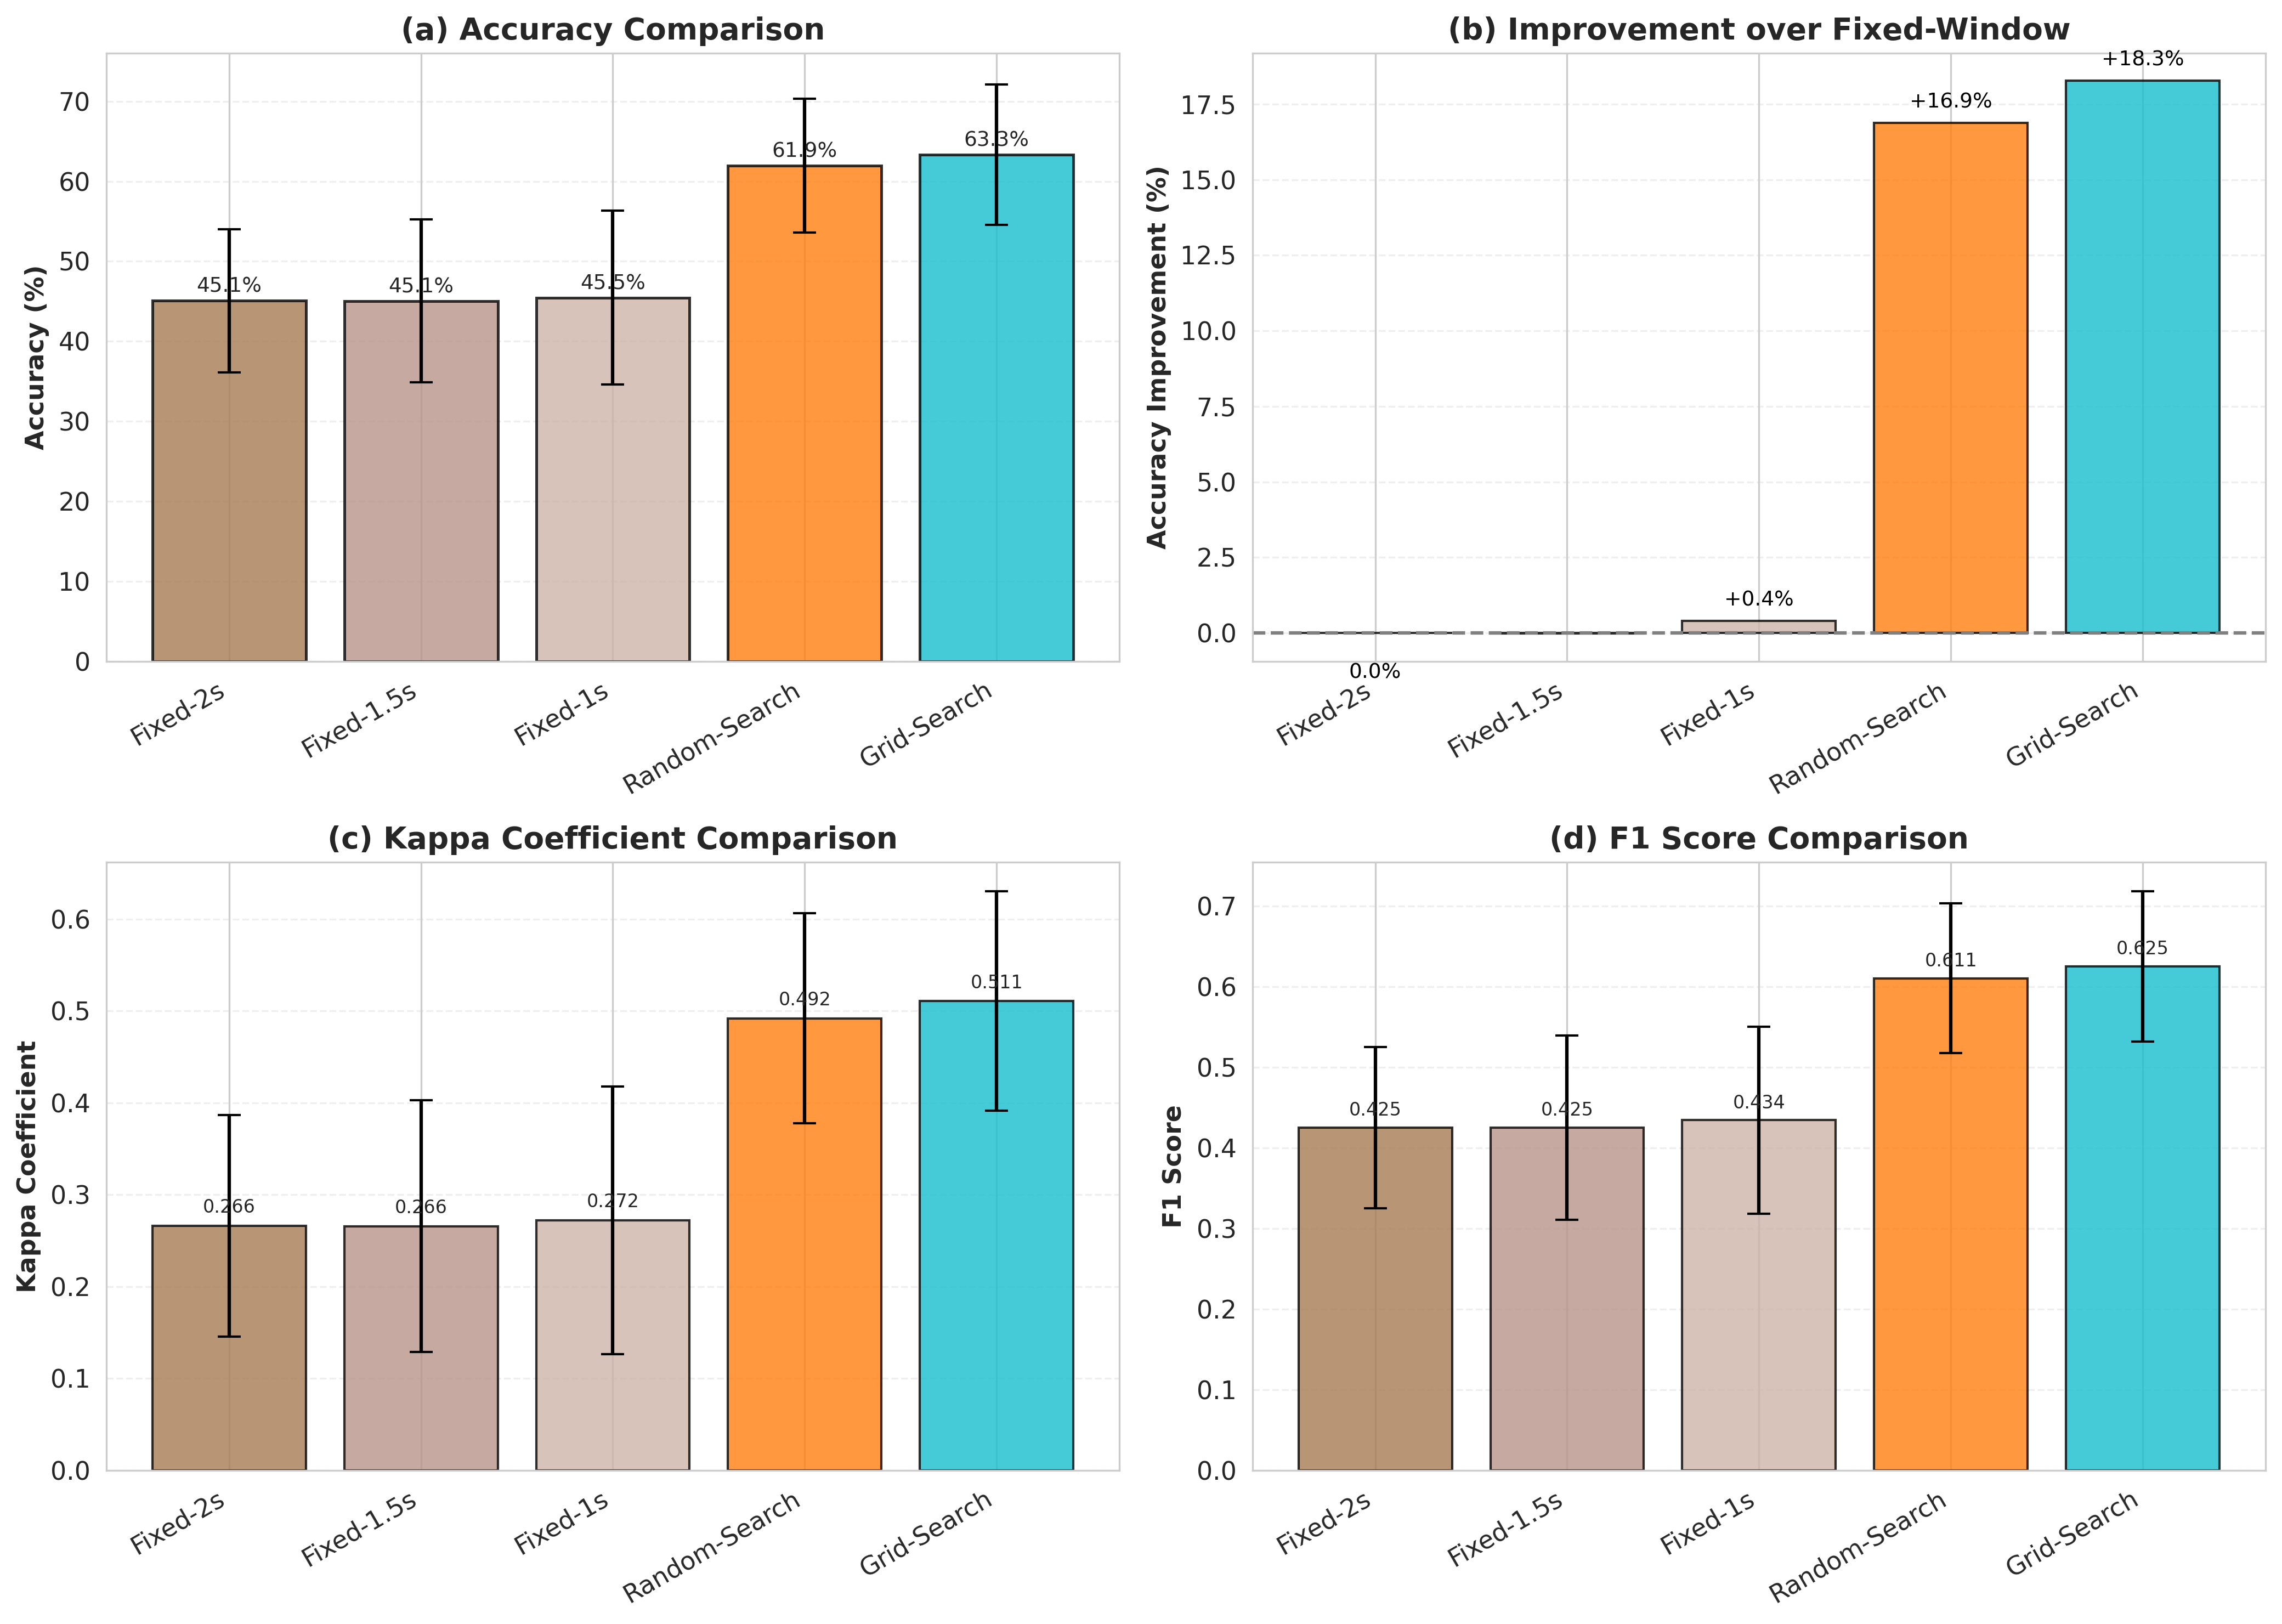
\includegraphics[height=0.8\textheight]{figures/baseline/01_performance_comparison.png}
\end{frame}

\begin{frame}{基线方法稳定性分析}
    \begin{columns}[T]
        \begin{column}{0.5\textwidth}
            \centering
            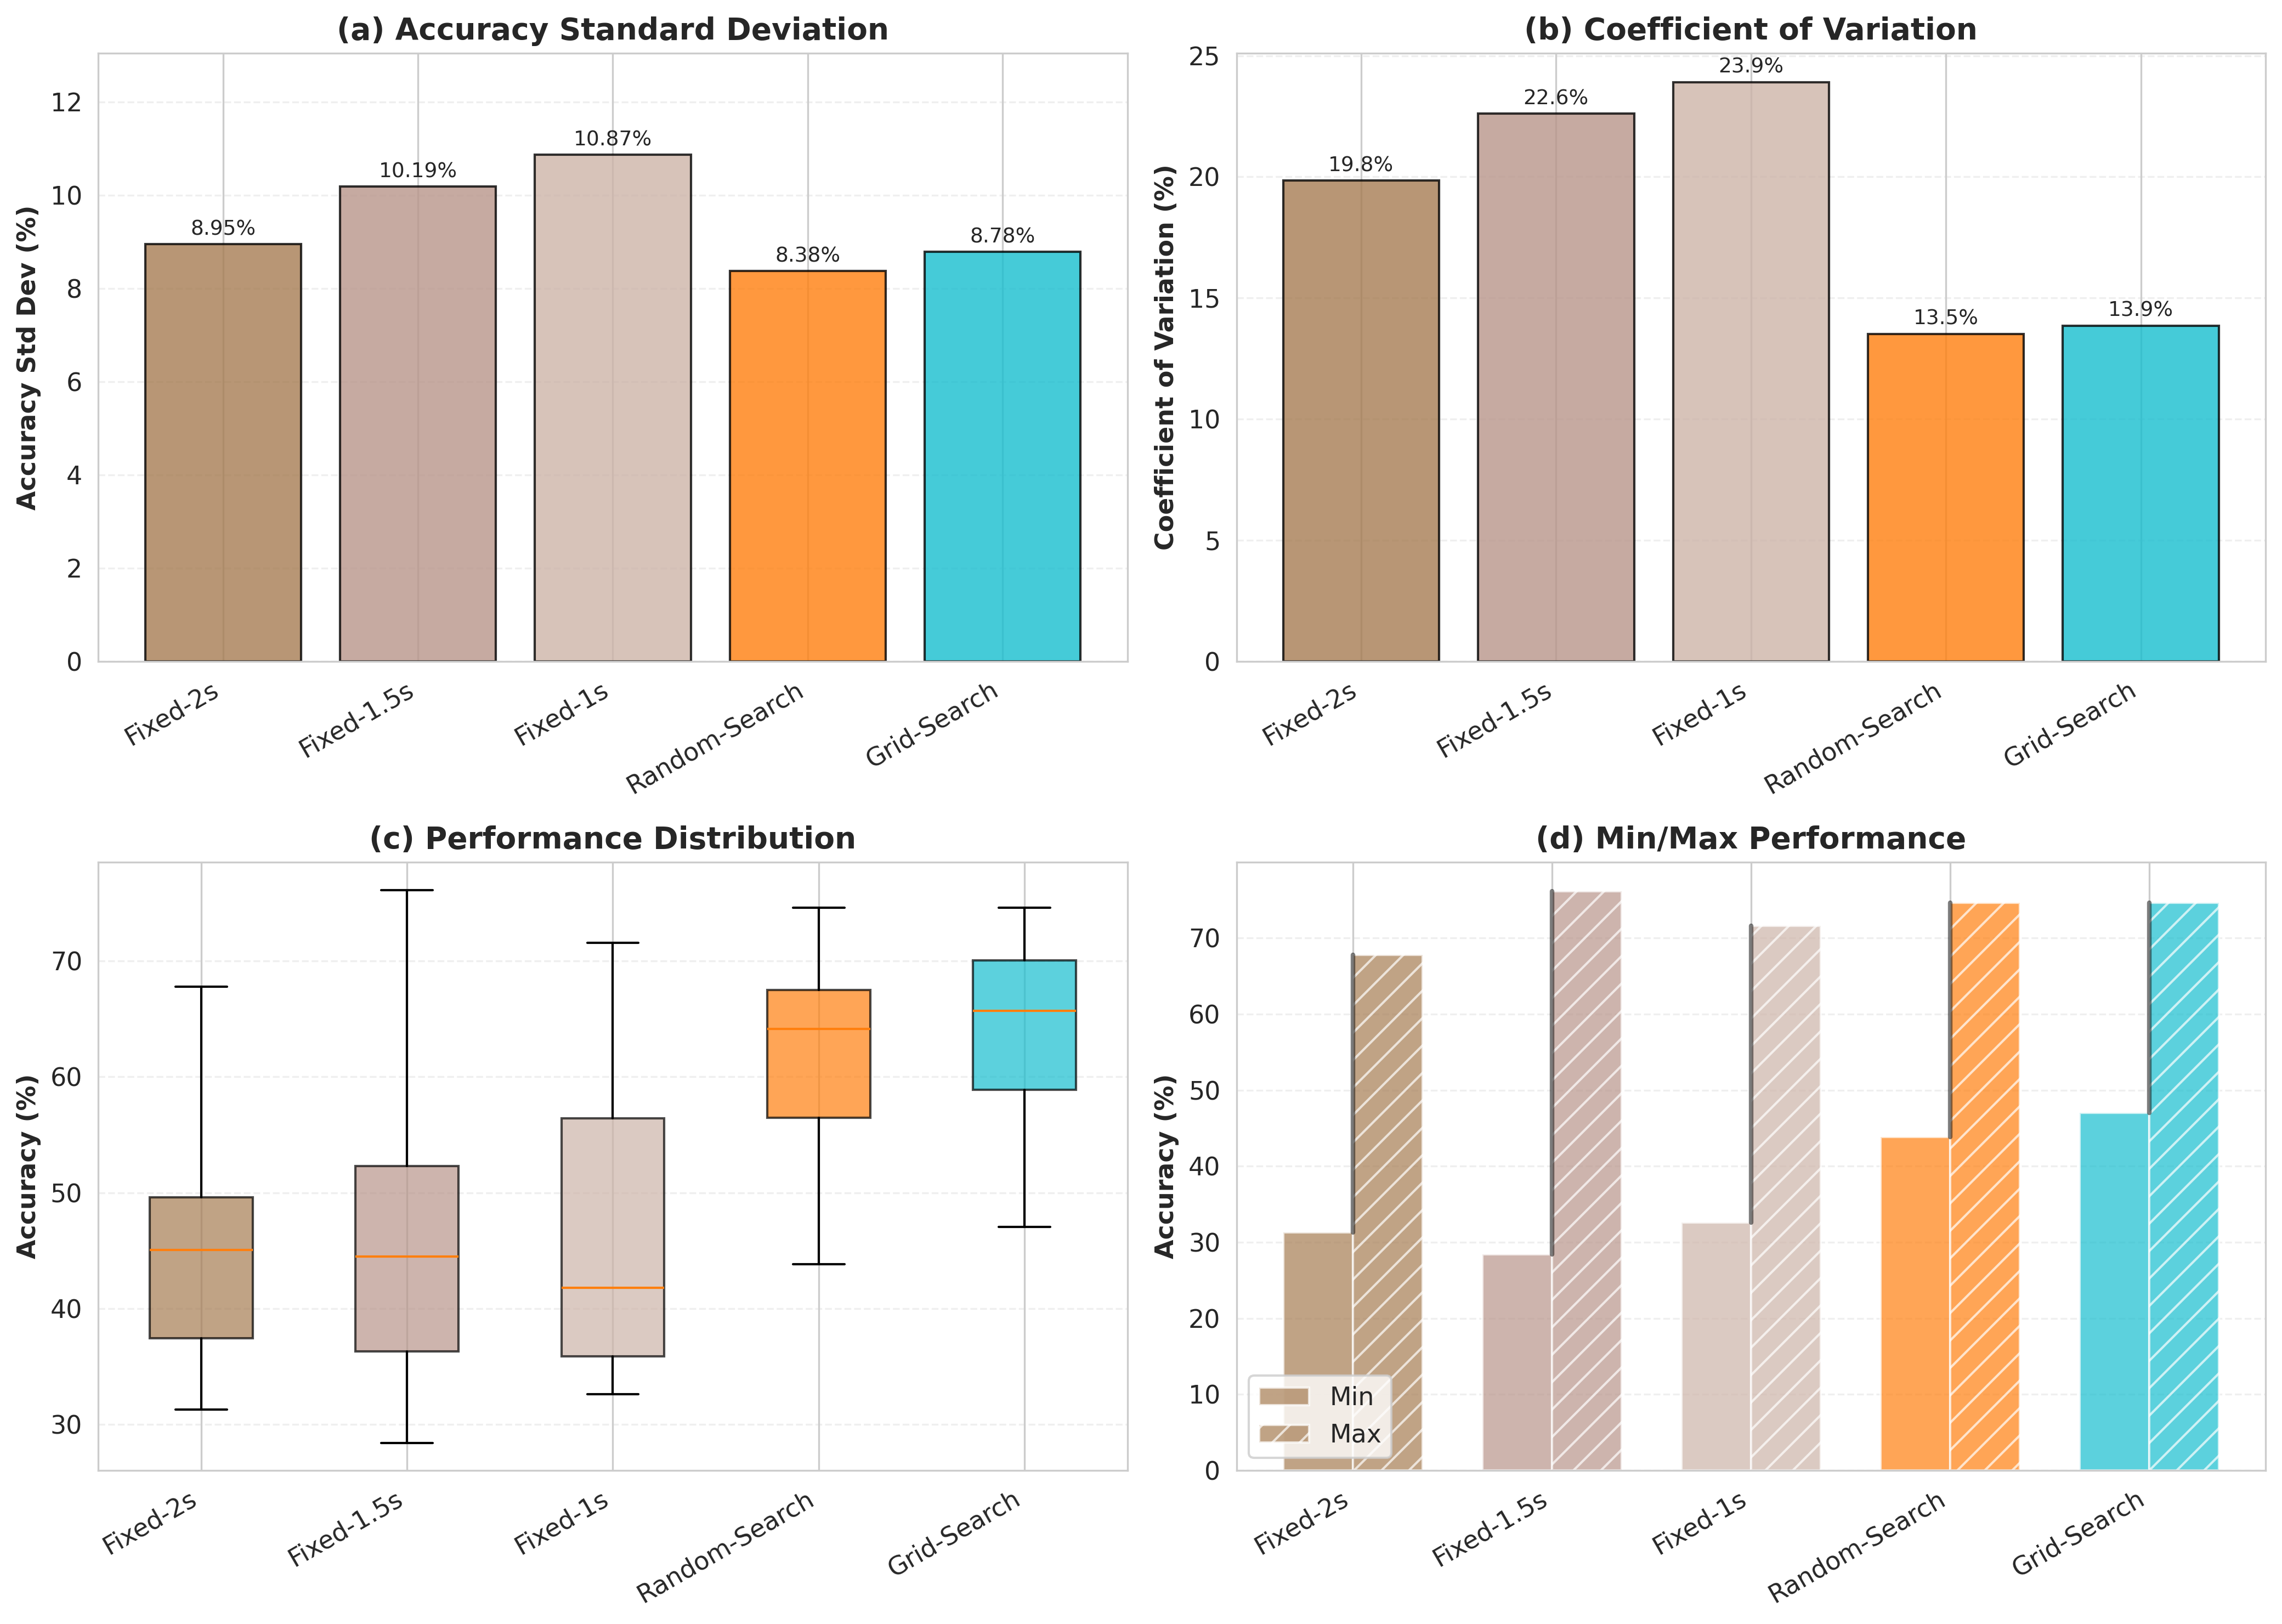
\includegraphics[height=0.7\textheight]{figures/baseline/01_stability_analysis.png}
            \vspace{-0.5em}
            \parbox{0.9\textwidth}{\footnotesize 图：基线方法稳定性箱线图}
        \end{column}

        \begin{column}{0.5\textwidth}
            \centering
            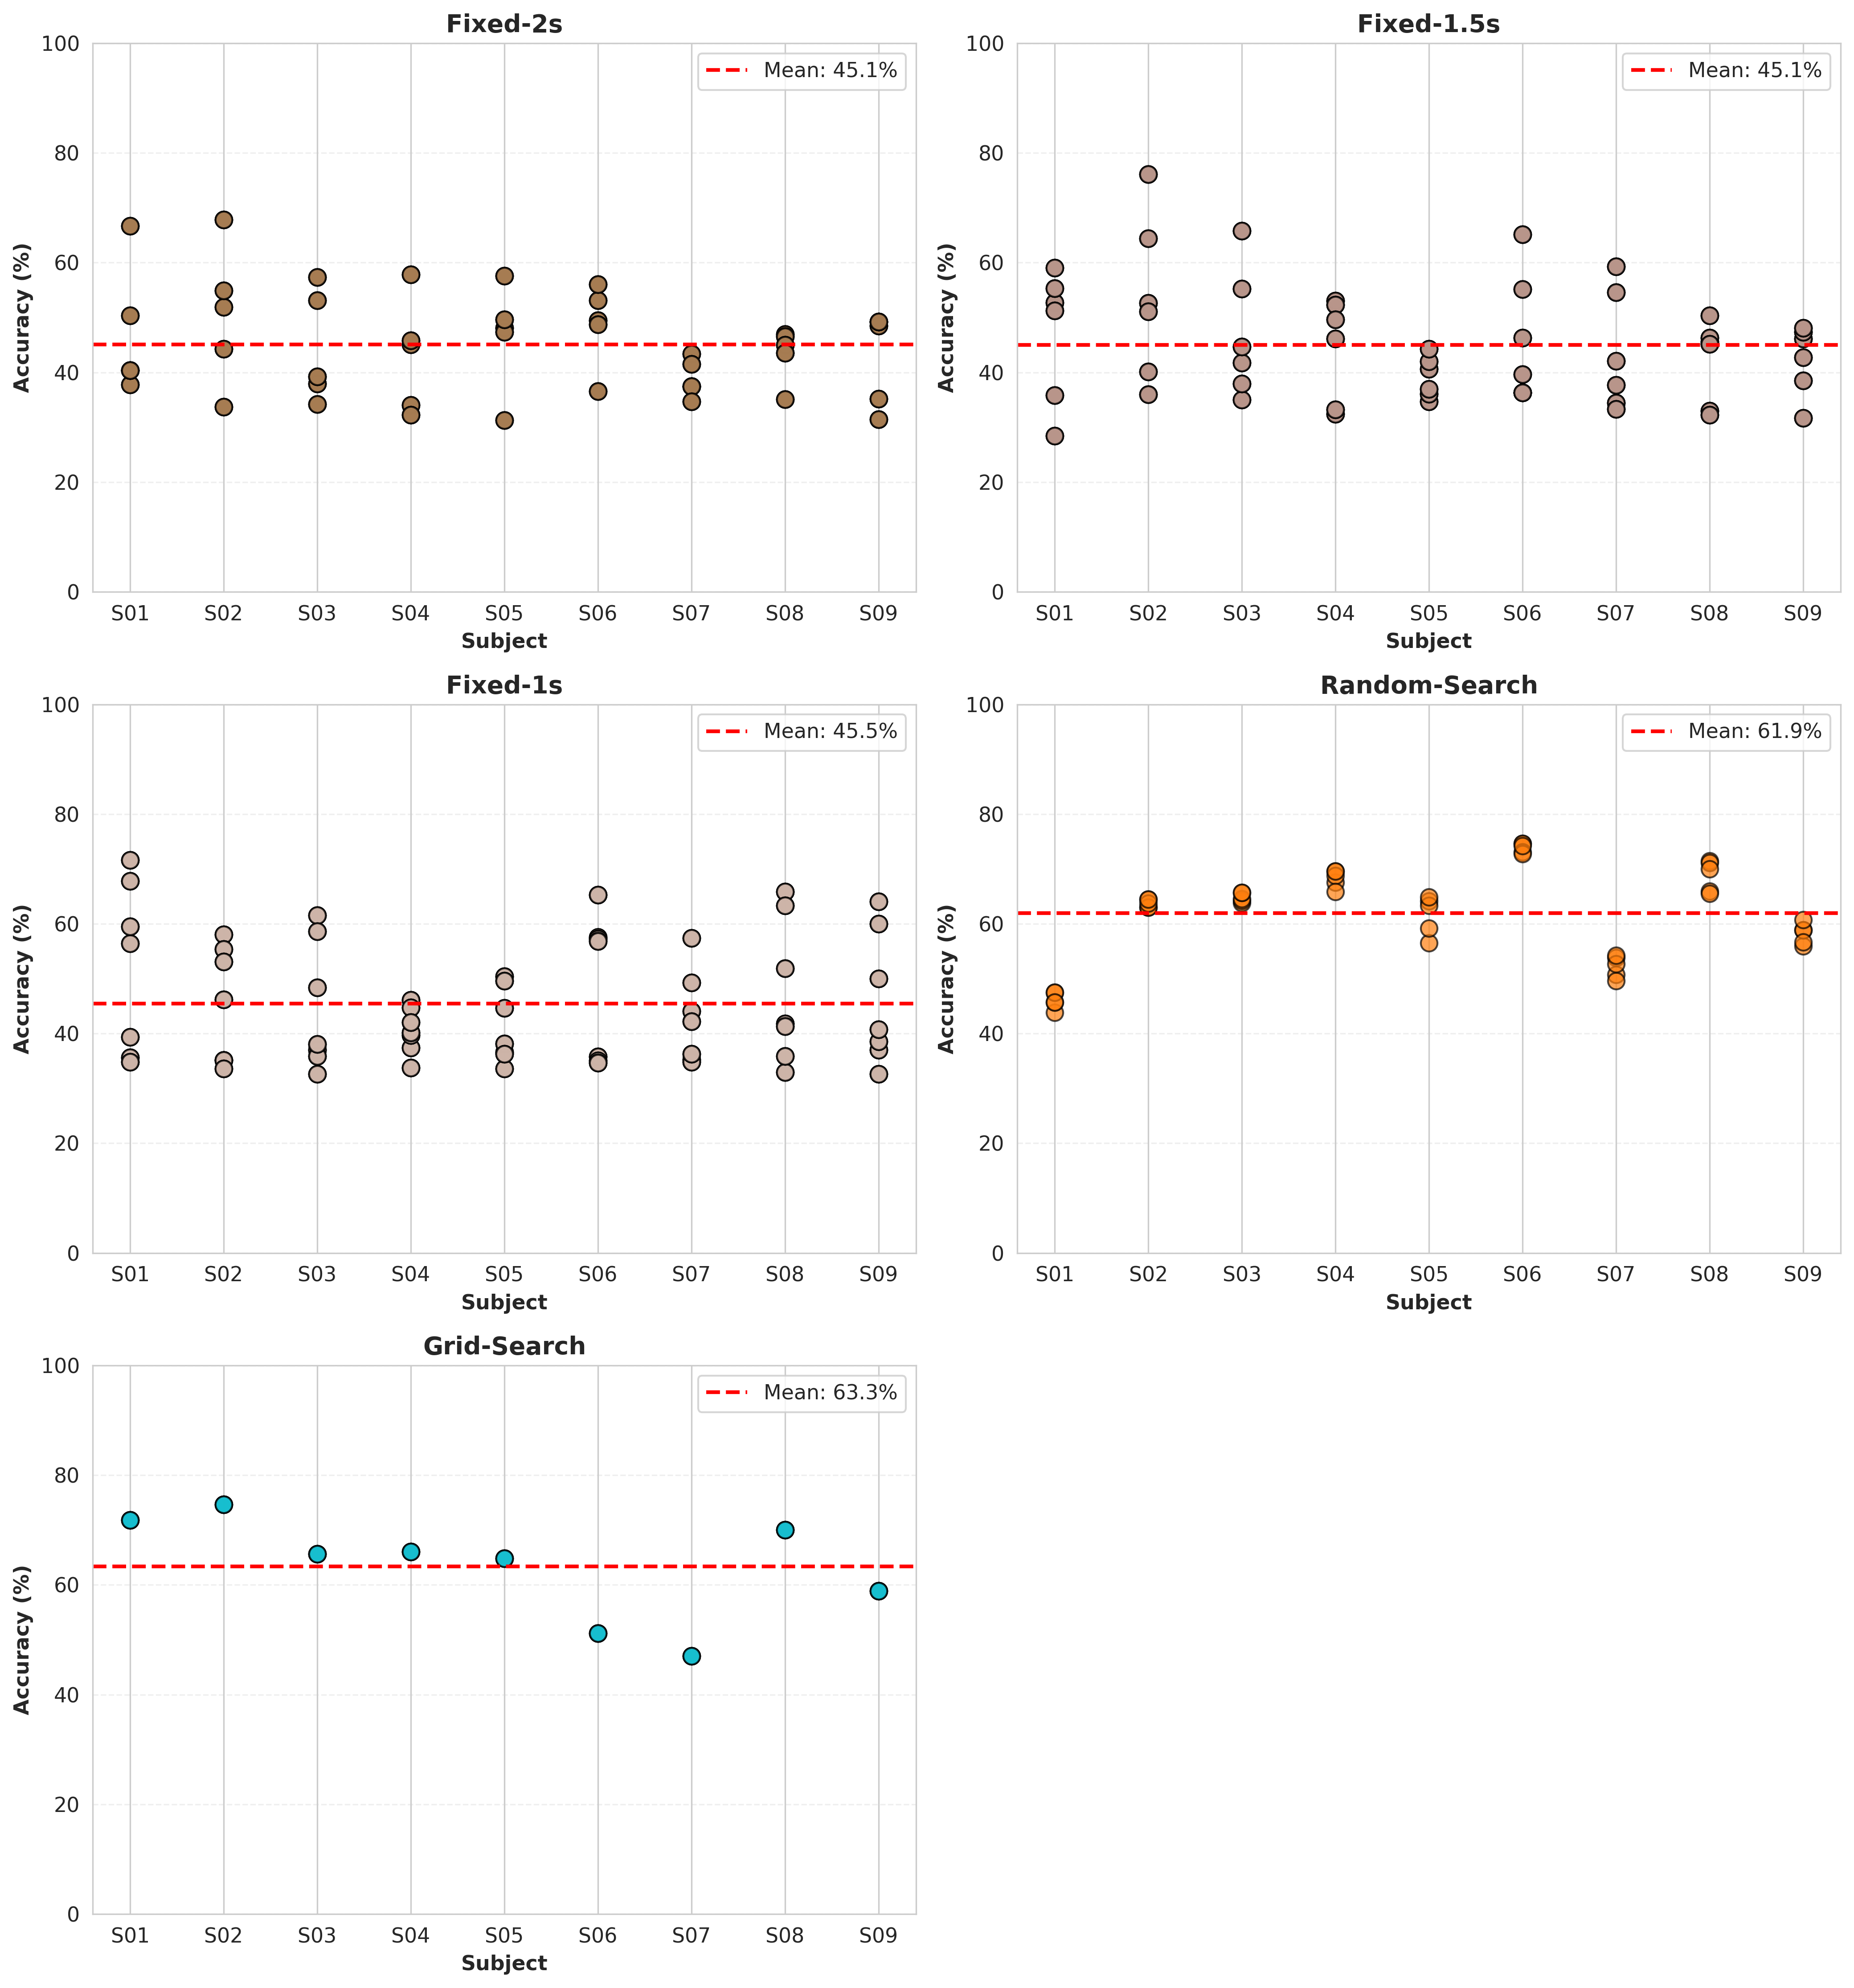
\includegraphics[height=0.7\textheight]{figures/baseline/01_subject_distribution.png}
            \vspace{-0.5em}
            \parbox{0.9\textwidth}{\footnotesize 图：被试级别性能热力图}
        \end{column}
    \end{columns}


\end{frame}

% ==================== Q-Learning 与基线方法对比 ====================
\begin{frame}{Q-Learning 方法与基线方法整体对比}
    \centering
    \vspace{-0.5em}
    \begin{table}
        \centering
        \begin{tabular}{lccccc}
            \toprule
            \textbf{Method} & \textbf{Acc (\%)} & \textbf{Kappa} & \textbf{F1} & \textbf{Std (\%)} & \textbf{$t_{start}$} \\
            \midrule
            Grid-Search & \textbf{63.35} & \textbf{0.5107} & \textbf{0.6252} & 8.78 & 2.27 \\
            \rowcolor{lightblue}
            \textbf{\color{primaryblue}Standard Q-Learning} & \textbf{62.68} & \textbf{0.5019} & \textbf{0.6201} & \textbf{8.20} & 2.29 \\
            Dueling Q-Learning & 62.74 & 0.5029 & 0.6204 & 8.26 & 2.27 \\
            \rowcolor{lightblue}
            DQN & 62.70 & 0.5022 & 0.6200 & 9.21 & 2.23 \\
            Double Q-Learning & 61.86 & 0.4909 & 0.6103 & 8.42 & 2.17 \\
            \rowcolor{lightblue}
            Dueling Double Q & 61.73 & 0.4894 & 0.6094 & 9.11 & 2.17 \\
            Random-Search & 61.95 & 0.4920 & 0.6106 & 8.38 & 2.20 \\
            \bottomrule
        \end{tabular}
    \end{table}


    \begin{alertblock}{\normalsize 核心发现}
        \begin{itemize}
            \item \textbf{Standard Q-Learning 稳定性最优}：Std Dev = 8.20\%（所有方法最低）
            \item \textbf{与 Grid-Search 性能接近}：Δ = -0.67\%，但计算成本更低
            \item \textbf{复杂变体未带来收益}：Double/Dueling 性能反而下降
        \end{itemize}
    \end{alertblock}
\end{frame}

\begin{frame}{Q-Learning 与基线方法对比（可视化）}
    \centering
    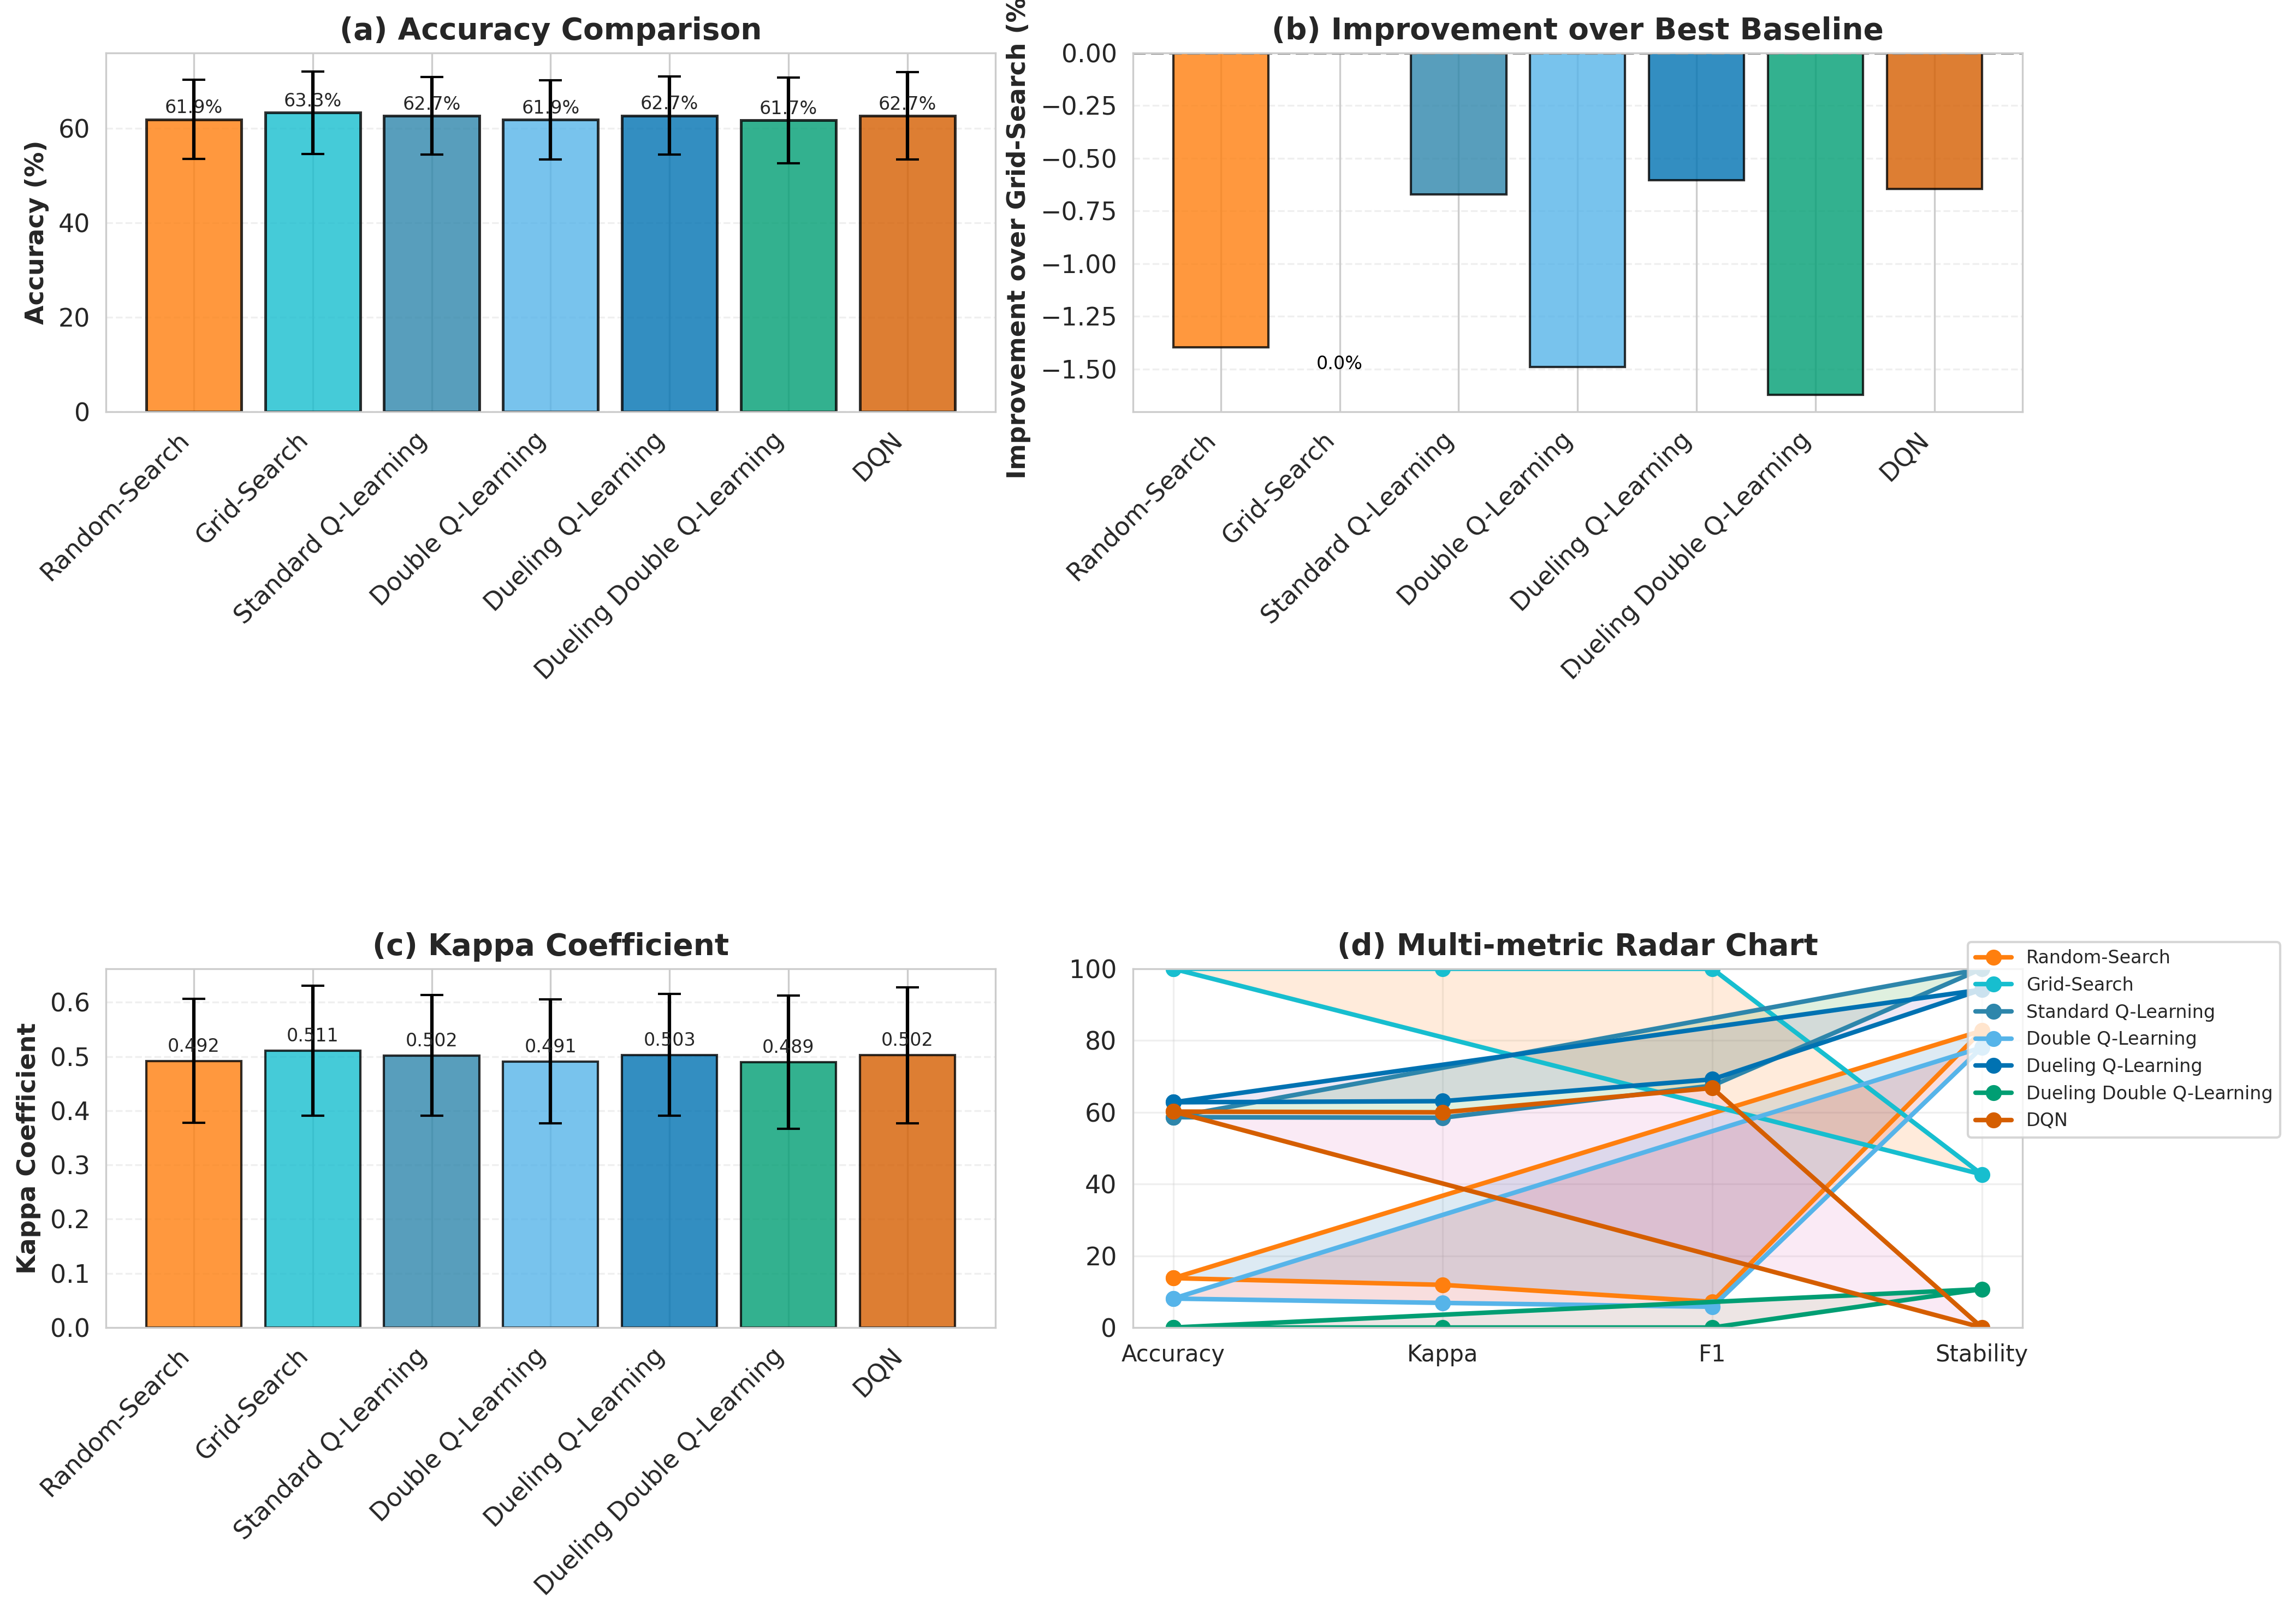
\includegraphics[height=0.7\textheight]{figures/q_vs_baseline/02_performance_comparison.png}
    \vspace{0.3em}
    \parbox{0.8\textwidth}{\footnotesize 图：Q-Learning 与基线方法性能对比}
\end{frame}

\begin{frame}{效应量分析与性能排名}
    \begin{columns}[T]
        \begin{column}{0.55\textwidth}
            \centering
            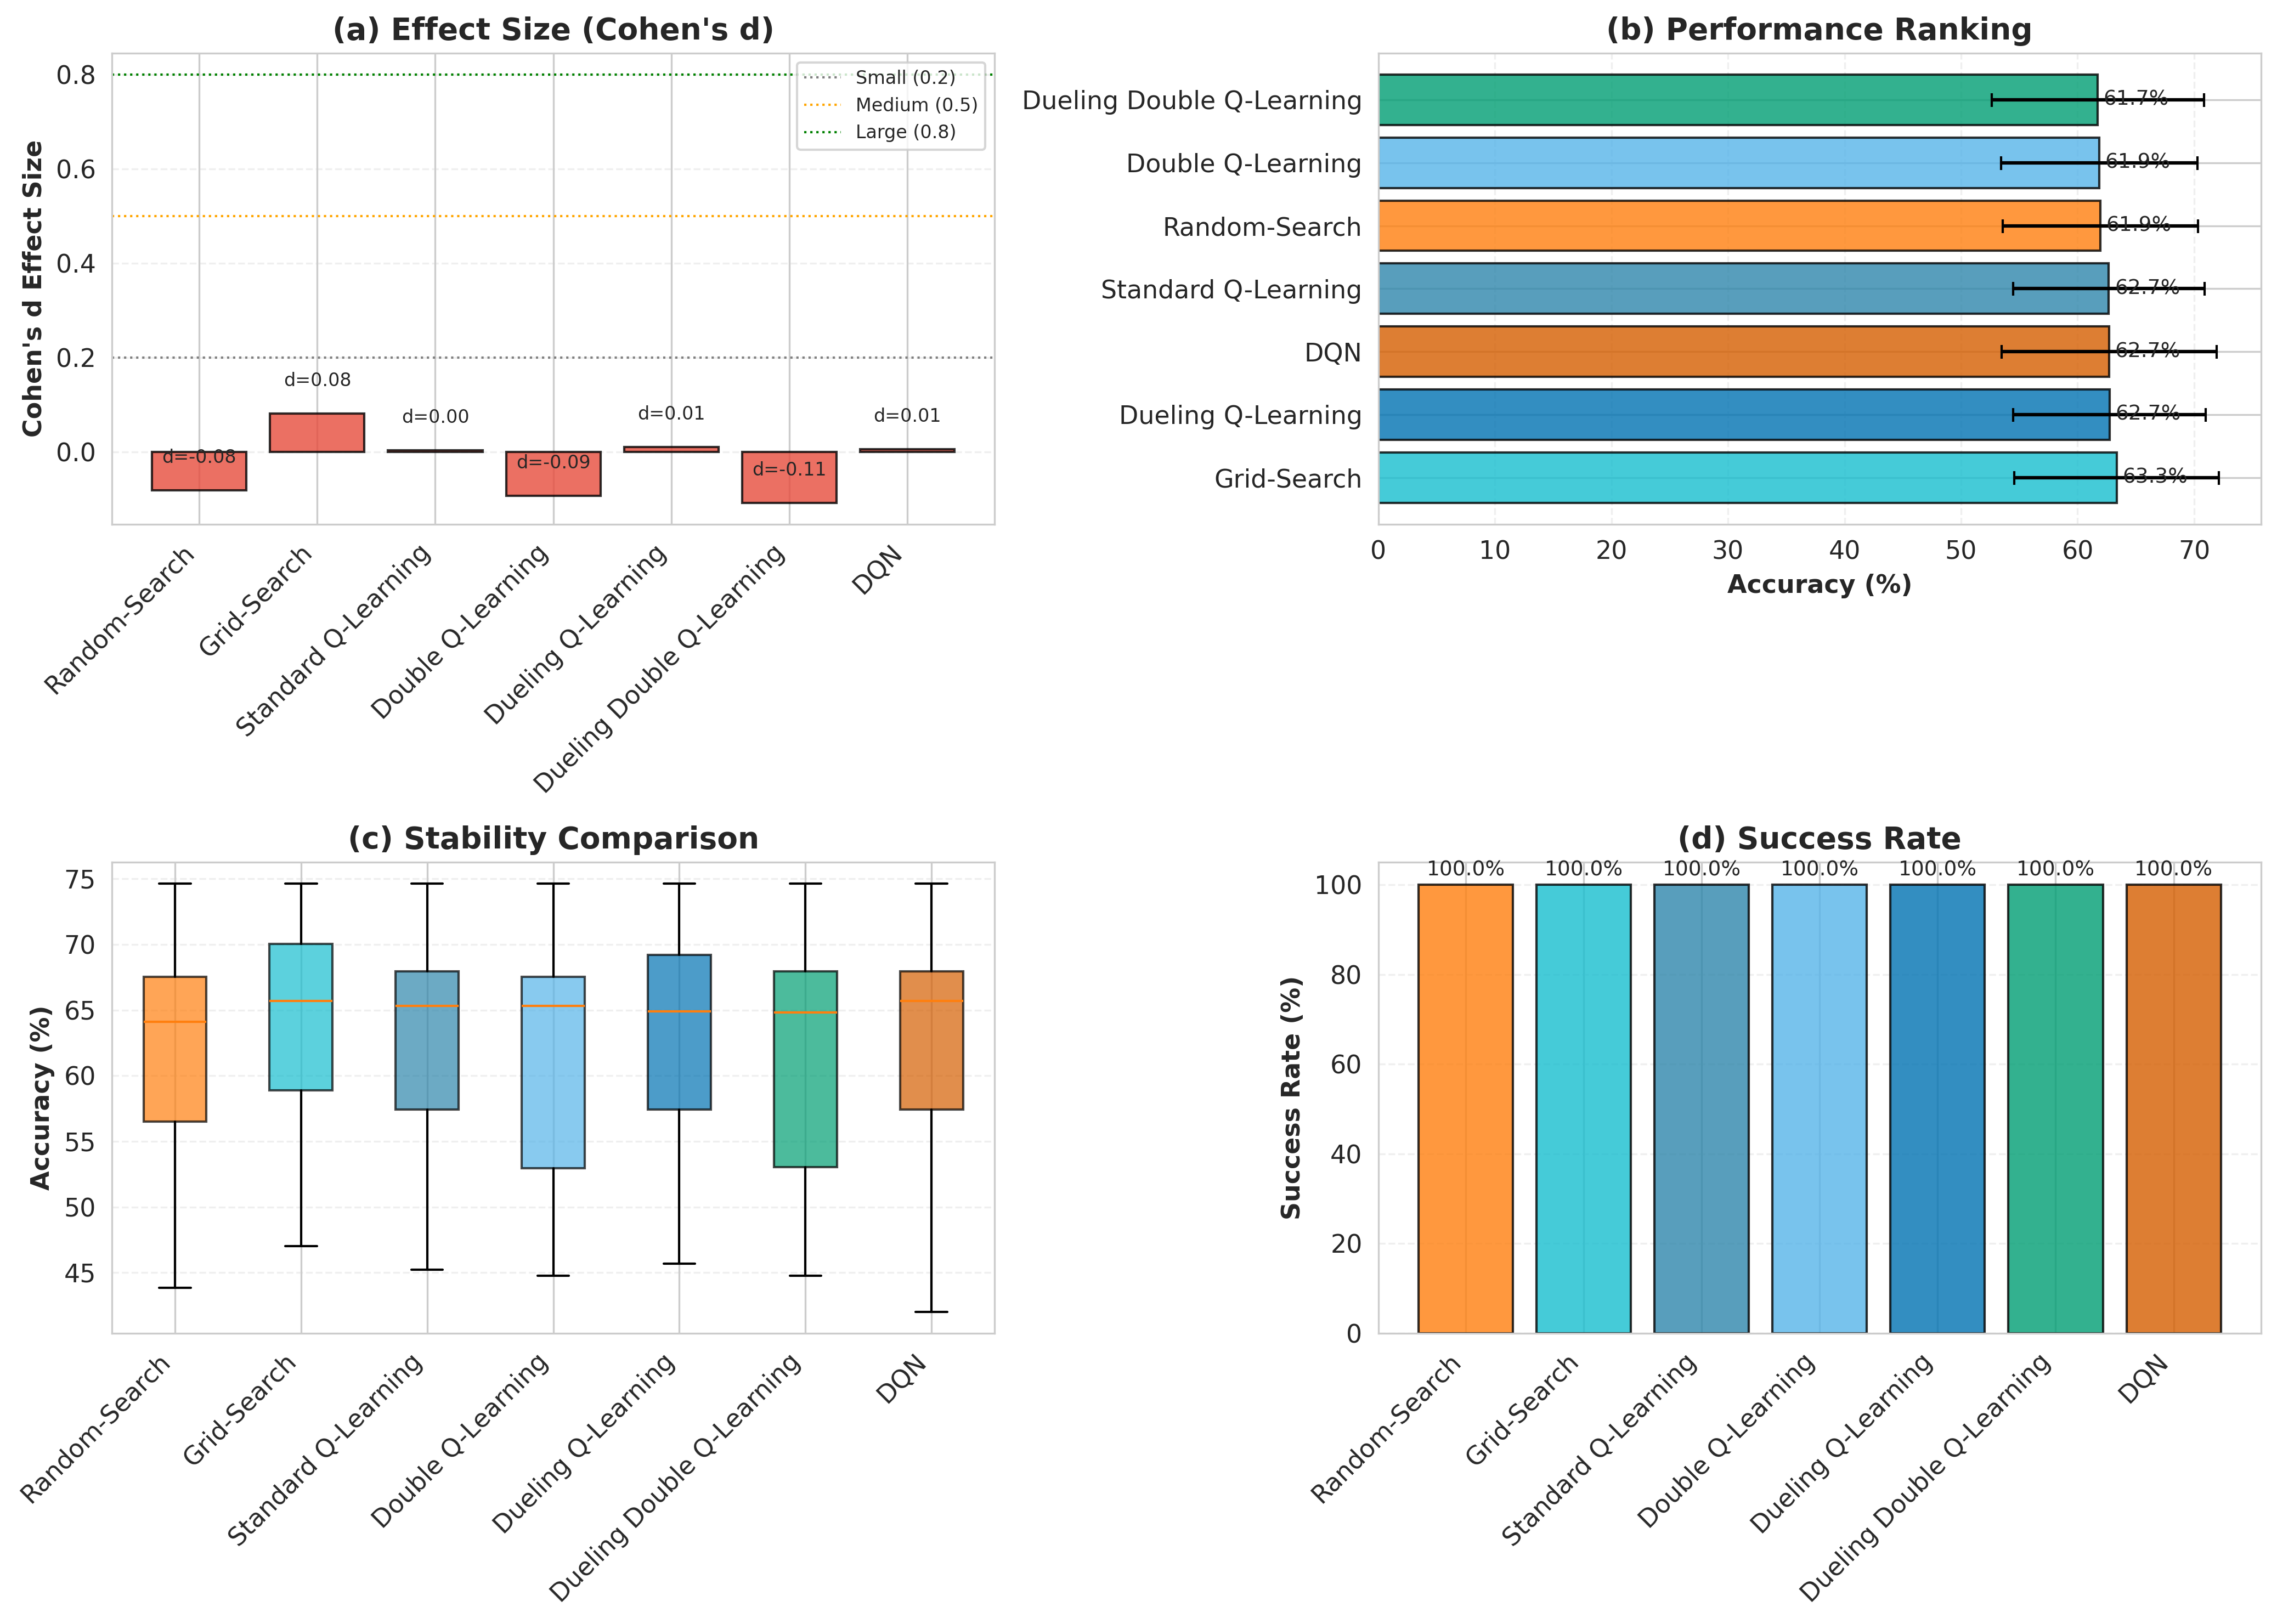
\includegraphics[height=0.6\textheight]{figures/q_vs_baseline/02_statistical_analysis.png}
            \vspace{-0.5em}
            \parbox{0.9\textwidth}{\footnotesize 图：Cohen's d 效应量与性能排名}
        \end{column}

        \begin{column}{0.45\textwidth}
            \begin{block}{\normalsize 效应量分析}
                以 Standard Q-Learning 为基准：
                \begin{itemize}
                    \item Grid-Search: $d = 0.08$（略优，小效应）
                    \item Random-Search: $d = -0.08$
                    \item Double Q-Learning: $d = -0.09$
                    \item Dueling Double Q: $d = -0.11$
                    \item DQN: $d = 0.01$（几乎无差异）
                \end{itemize}
            \end{block}

            \vspace{0.5em}

            \begin{exampleblock}{\normalsize 结论}
                所有效应量均在 $[-0.11, 0.08]$ 范围内，远小于 0.2 的小效应阈值。
            \end{exampleblock}
        \end{column}
    \end{columns}
\end{frame}

\begin{frame}{时间窗选择分析}
    \centering
    \vspace{-0.5em}
    \begin{table}
        \centering
        \Large
        \begin{tabular}{lccc}
            \toprule
            \textbf{Method} & \textbf{$t_{start}$ (s)} & \textbf{$t_{end}$ (s)} & \textbf{Length (s)} \\
            \midrule
            Standard Q-Learning & 2.29 & 3.17 & 0.88 \\
            \rowcolor{lightblue}
            DQN & 2.23 & 3.28 & 1.05 \\
            Grid-Search & 2.27 & 3.16 & 0.89 \\
            \bottomrule
        \end{tabular}
    \end{table}

    \vspace{0.5em}

    \begin{alertblock}{\normalsize 时间窗选择规律}
        \begin{itemize}
            \item \textbf{起始点集中}：2.17s–2.29s（ERD 典型起始时间）
            \item \textbf{结束点集中}：3.16s–3.28s（ERD 活跃期）
            \item \textbf{短窗口优势}：Grid-Search (0.89s) 和 Standard Q-Learning (0.88s) 选择更短窗口
        \end{itemize}
    \end{alertblock}
\end{frame}

\begin{frame}{时间窗与性能关系}
    \centering
    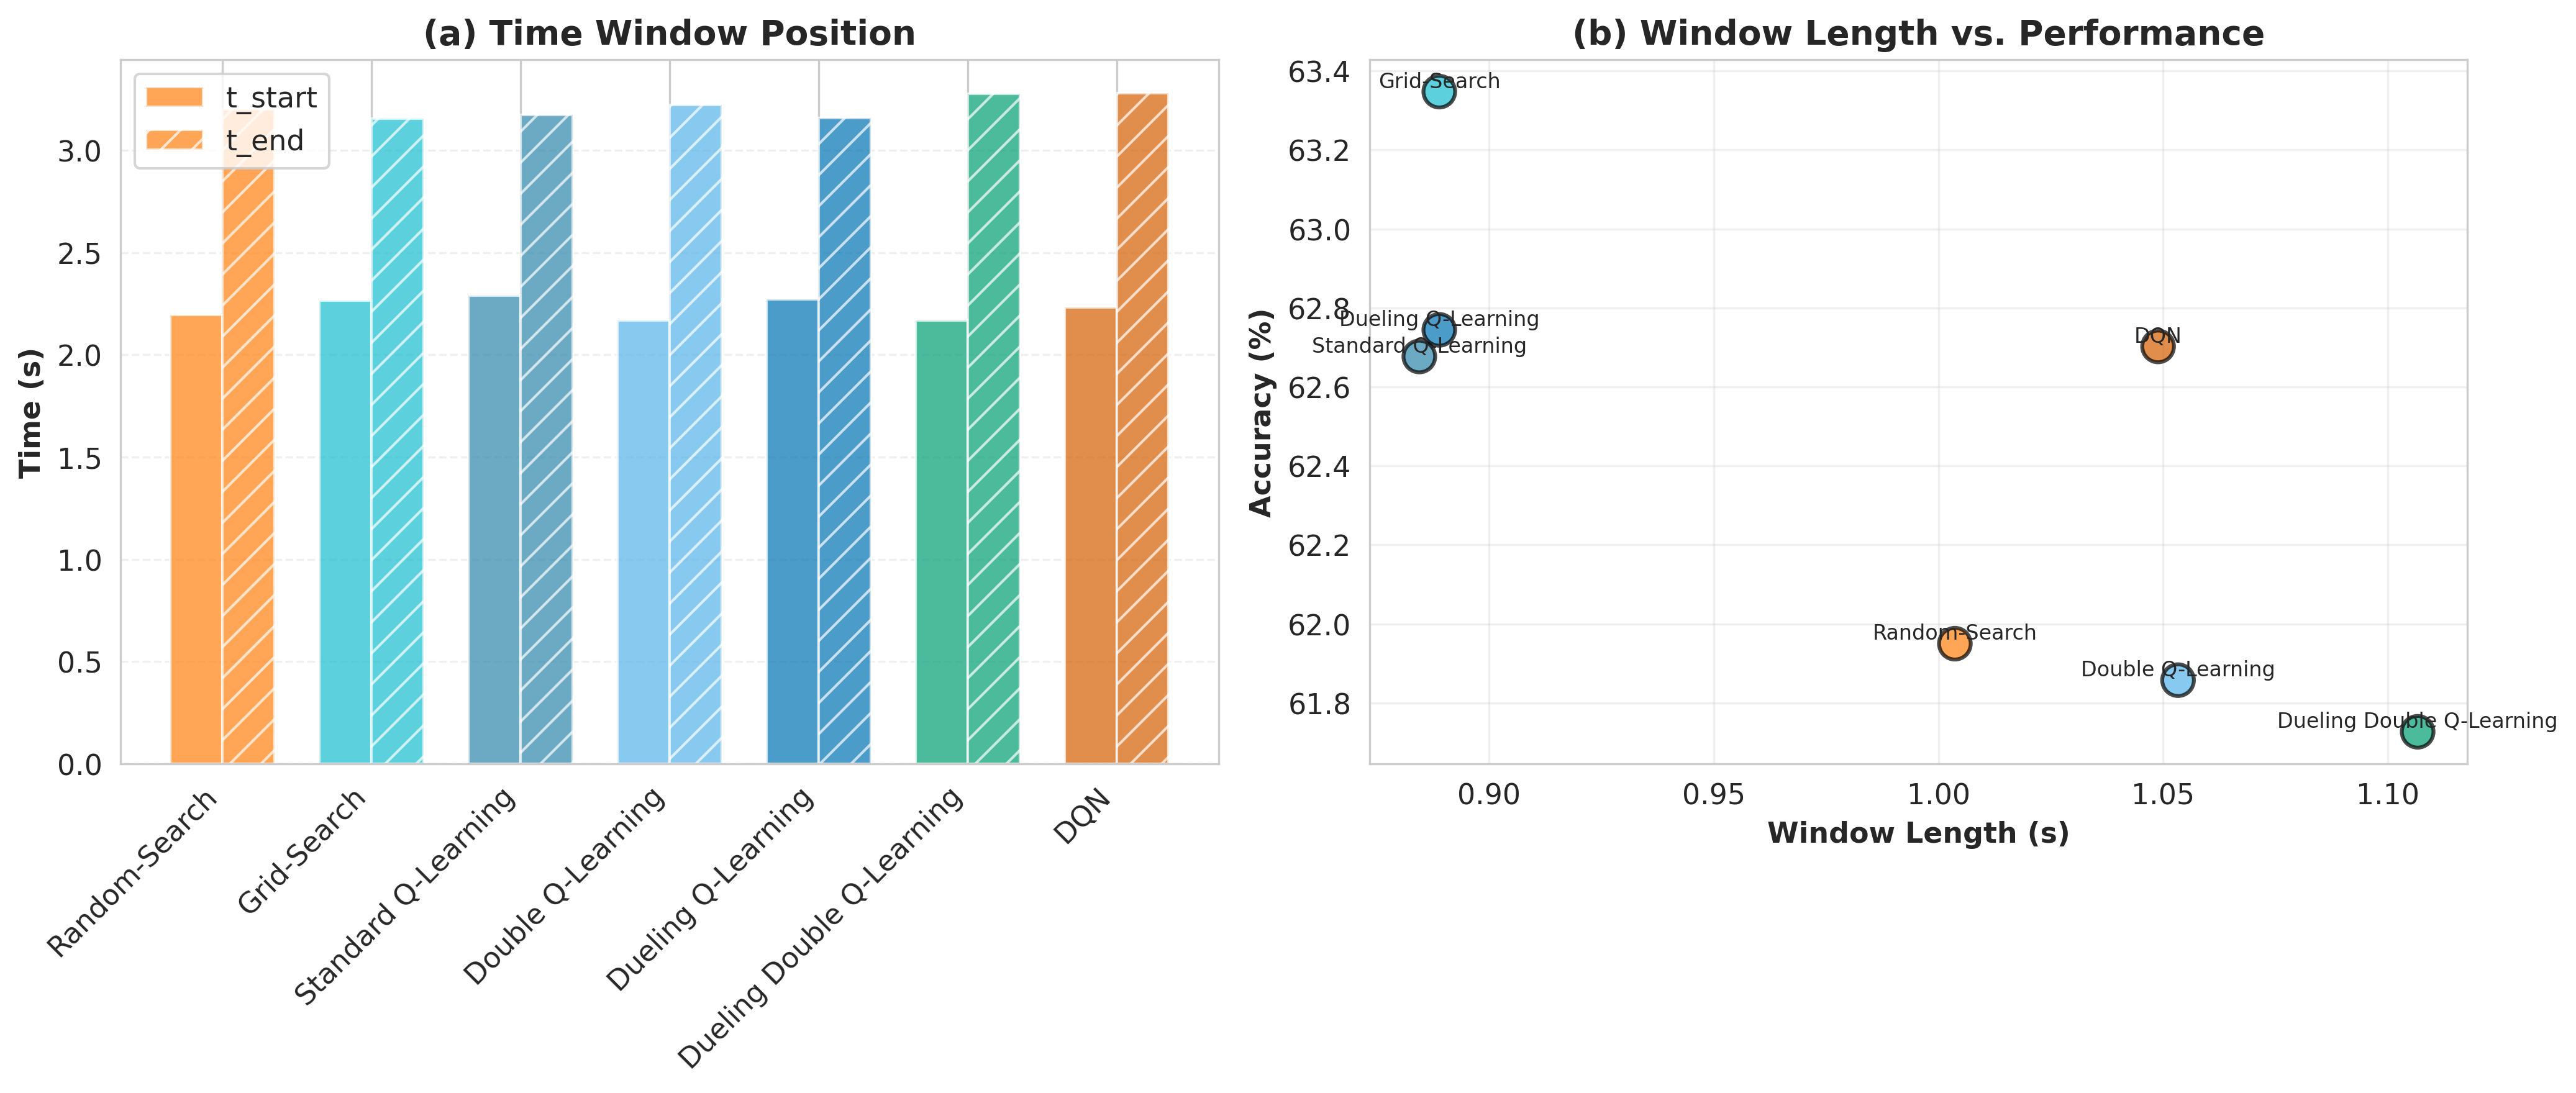
\includegraphics[height=0.7\textheight]{figures/q_vs_baseline/02_window_performance.png}
    \vspace{0.3em}
    \parbox{0.8\textwidth}{\footnotesize 图：窗口长度与性能关系散点图}
\end{frame}

% ==================== 表格型 Q-Learning 与 DQN 对比 ====================
\begin{frame}{表格型 Q-Learning vs DQN：整体性能}
    \centering
    \vspace{-0.5em}
    \begin{table}
        \centering
        \begin{tabular}{lcccccc}
            \toprule
            \textbf{Method} & \textbf{Acc (\%)} & \textbf{Kappa} & \textbf{F1} & \textbf{Std (\%)} & \textbf{$t_{start}$} & \textbf{$t_{end}$} \\
            \midrule
            \rowcolor{lightblue}
            \textbf{\color{primaryblue}Standard Q-Learning} & \textbf{62.68} & 0.5019 & 0.6201 & \textbf{8.20} & 2.29 & 3.17 \\
            DQN & \textbf{62.70} & 0.5022 & 0.6200 & 9.21 & 2.23 & 3.28 \\
            \textbf{Δ (Q - DQN)} & \textbf{-0.02} & -0.0003 & +0.0001 & \textbf{-1.01} & +0.06 & -0.11 \\
            \bottomrule
        \end{tabular}
    \end{table}

    \vspace{0.5em}

    \begin{alertblock}{\normalsize 核心发现}
        \begin{itemize}
            \item \textbf{\color{accentgreen}准确率差异极小}：仅 -0.02\%，统计学上可忽略
            \item \textbf{\color{accentgreen}稳定性优势}：标准差相对降低 10.97\%
            \item \textbf{时间窗选择}：Table Q 选择更短但信息密度更高的窗口 (0.88s vs 1.05s)
        \end{itemize}
    \end{alertblock}
\end{frame}

\begin{frame}{Table Q vs DQN 性能对比（可视化）}
    \centering
    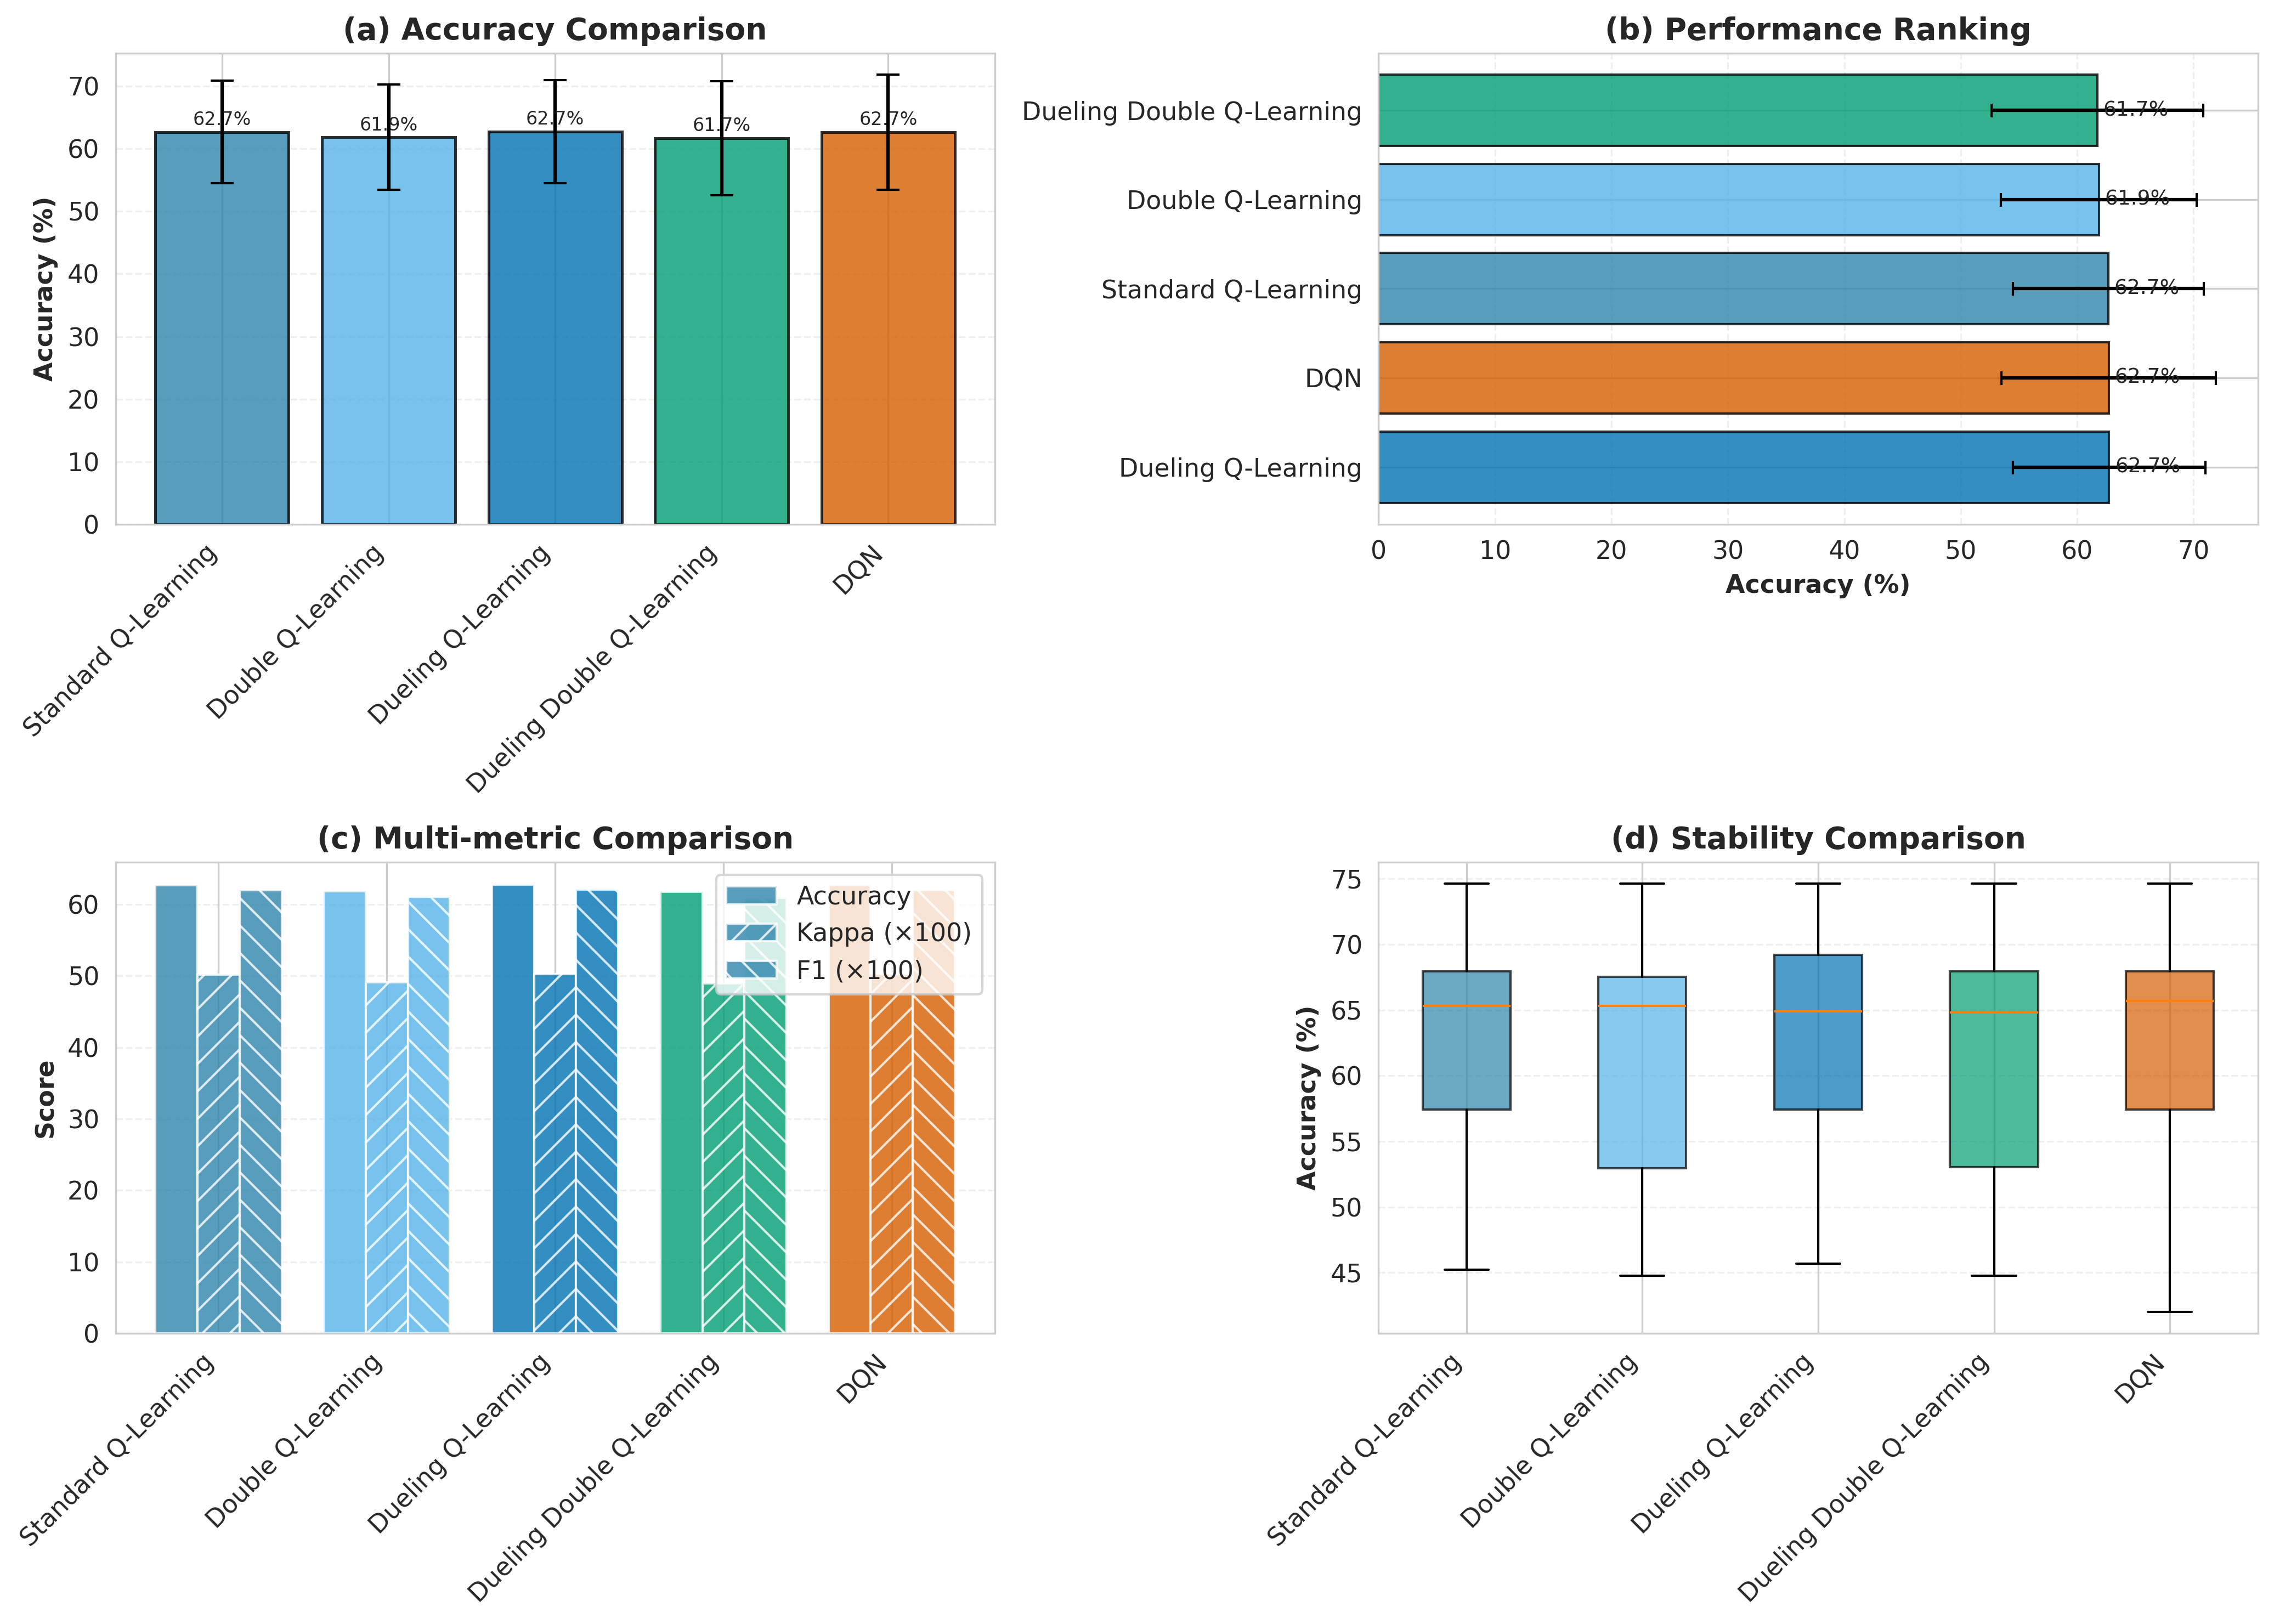
\includegraphics[height=0.7\textheight]{figures/q_internal/03_performance_comparison.png}
    \vspace{0.3em}
    \parbox{0.8\textwidth}{\footnotesize 图：Table Q vs DQN 性能对比}
\end{frame}

\begin{frame}{被试级别性能对比}
    \centering
    \vspace{-0.5em}
    \begin{table}
        \centering
        \footnotesize
        \begin{tabular}{lcccccc}
            \toprule
            \textbf{Sub} & \textbf{Table Q} & \textbf{DQN} & \textbf{Δ} & \textbf{Table Q $\kappa$} & \textbf{DQN $\kappa$} & \textbf{Δ$\kappa$} \\
            \midrule
            S01 & 64.47 & 65.71 & -1.24 & 0.5260 & 0.5435 & -0.018 \\
            \rowcolor{lightblue}
            S02 & 58.37 & 56.74 & +1.63 & 0.4780 & 0.4233 & +0.055 \\
            S03 & 68.89 & 71.70 & -2.81 & 0.5849 & 0.6226 & -0.038 \\
            \rowcolor{lightblue}
            S04 & 51.91 & 51.15 & +0.76 & 0.3590 & 0.3469 & +0.012 \\
            S05 & 65.42 & 65.27 & +0.15 & 0.5389 & 0.5368 & +0.002 \\
            \rowcolor{lightblue}
            S06 & 47.03 & 45.21 & +1.82 & 0.2952 & 0.2625 & +0.033 \\
            S07 & 65.46 & 65.61 & -0.15 & 0.5395 & 0.5416 & -0.002 \\
            \rowcolor{lightblue}
            S08 & 73.56 & 74.62 & -1.06 & 0.6470 & 0.6611 & -0.014 \\
            S09 & 68.69 & 68.27 & +0.42 & 0.5824 & 0.5769 & +0.006 \\
            \bottomrule
        \end{tabular}
    \end{table}

    \vspace{0.3em}

    \begin{exampleblock}{\normalsize 发现}
        \begin{itemize}
            \item \textbf{优劣分布均衡}：Table Q 在 5 名被试上优于或持平 DQN
            \item \textbf{低表现被试优势}：S06 上 Table Q 优于 DQN (+1.82\%)
            \item \textbf{高表现被试差距小}：S03、S08 差距 < 3\%
        \end{itemize}
    \end{exampleblock}
\end{frame}

\begin{frame}{被试级别性能对比（可视化）}
    \centering
    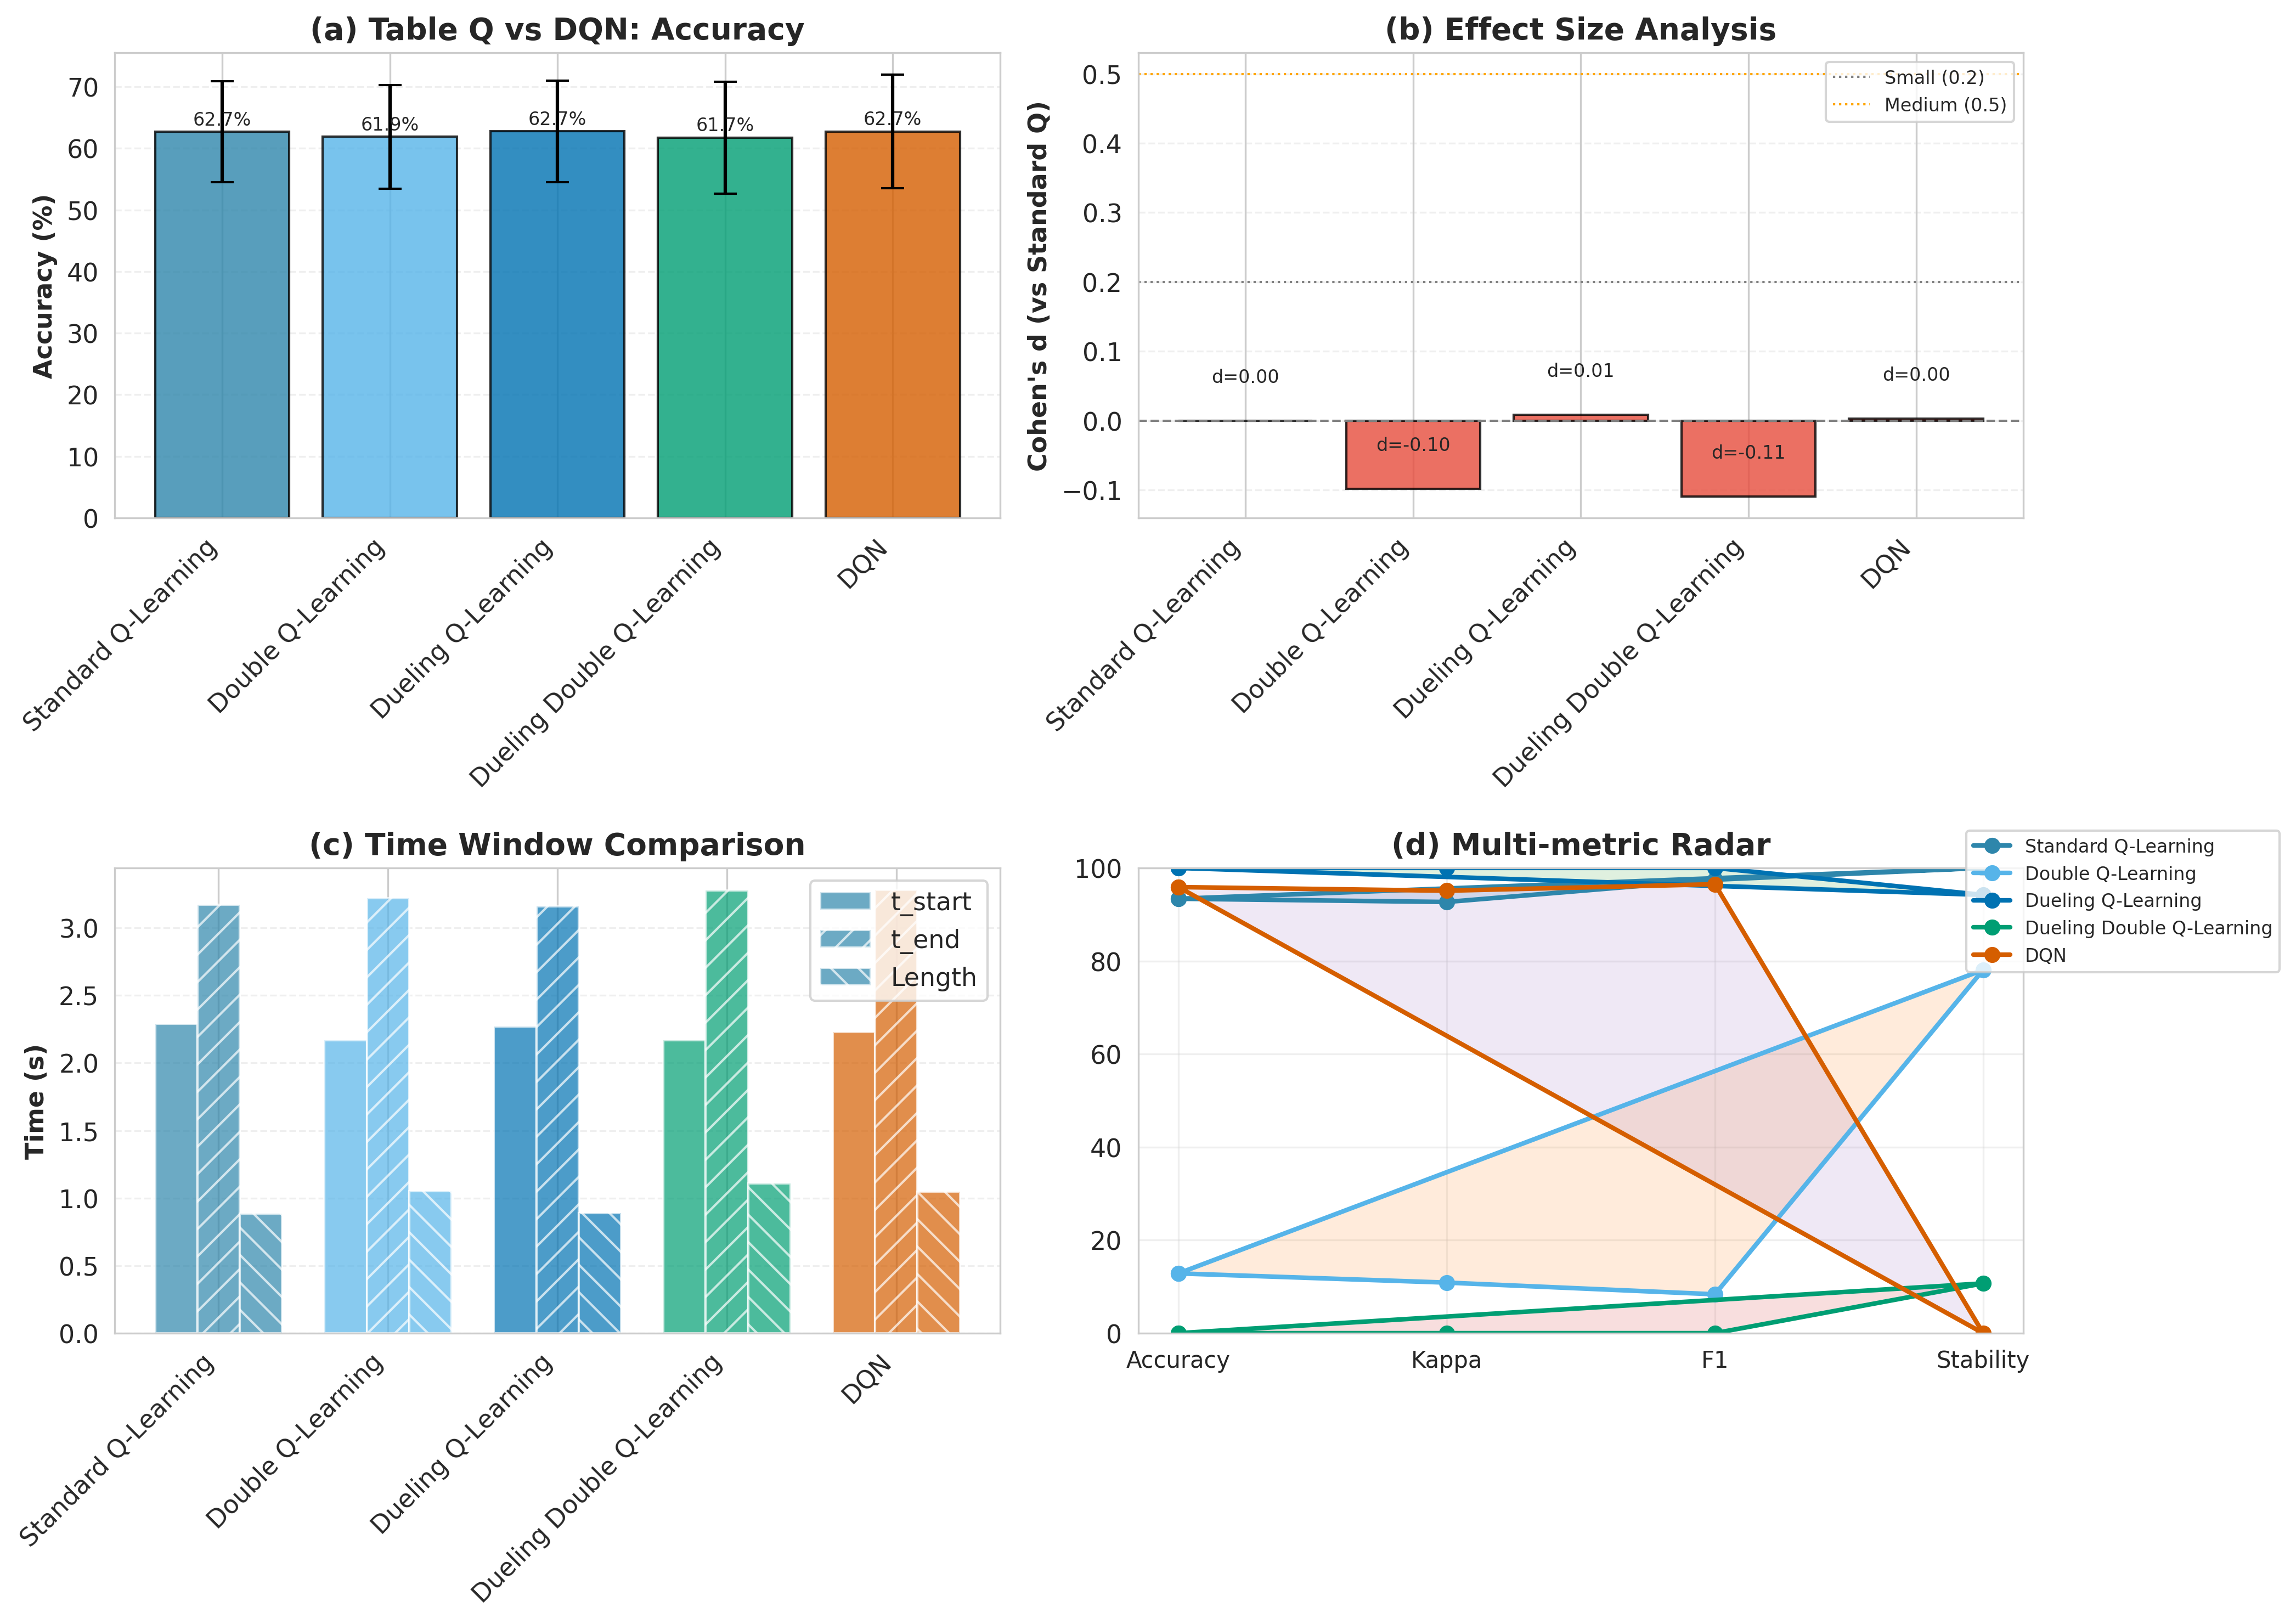
\includegraphics[height=0.7\textheight]{figures/q_internal/03_table_q_vs_dqn.png}
    \vspace{0.3em}
    \parbox{0.8\textwidth}{\footnotesize 图：被试级别性能对比}
\end{frame}

\begin{frame}{统计显著性检验}
    \begin{columns}[T]
        \begin{column}{0.48\textwidth}
            \begin{alertblock}{\normalsize 配对样本 t 检验}
                \begin{itemize}
                    \item \textbf{零假设} $H_0$：$\mu_d = 0$（无显著差异）
                    \item \textbf{备择假设} $H_1$：$\mu_d \neq 0$
                \end{itemize}

                \vspace{0.5em}

                \textbf{检验结果}：
                \begin{itemize}
                    \item $t$ 统计量：$t(8) = \textbf{-0.024}$
                    \item $p$ 值：\textbf{\color{accentgreen}$p = 0.981$}
                    \item 95\% CI：$[-2.01\%, 1.97\%]$
                    \item Cohen's $d = \textbf{-0.003}$
                \end{itemize}
            \end{alertblock}
        \end{column}

        \begin{column}{0.48\textwidth}
            \begin{exampleblock}{\normalsize 结果解读}
                \begin{itemize}
                    \item $p = 0.981 > 0.05$，\textbf{\color{accentgreen}不能拒绝零假设}
                    \item 效应量 $d = -0.003$ 远小于 0.2
                    \item \textbf{结论}：两种方法性能差异在统计学上不显著
                \end{itemize}
            \end{exampleblock}
        \end{column}
    \end{columns}
\end{frame}

\begin{frame}{模型训练性能可视化}
    \centering
    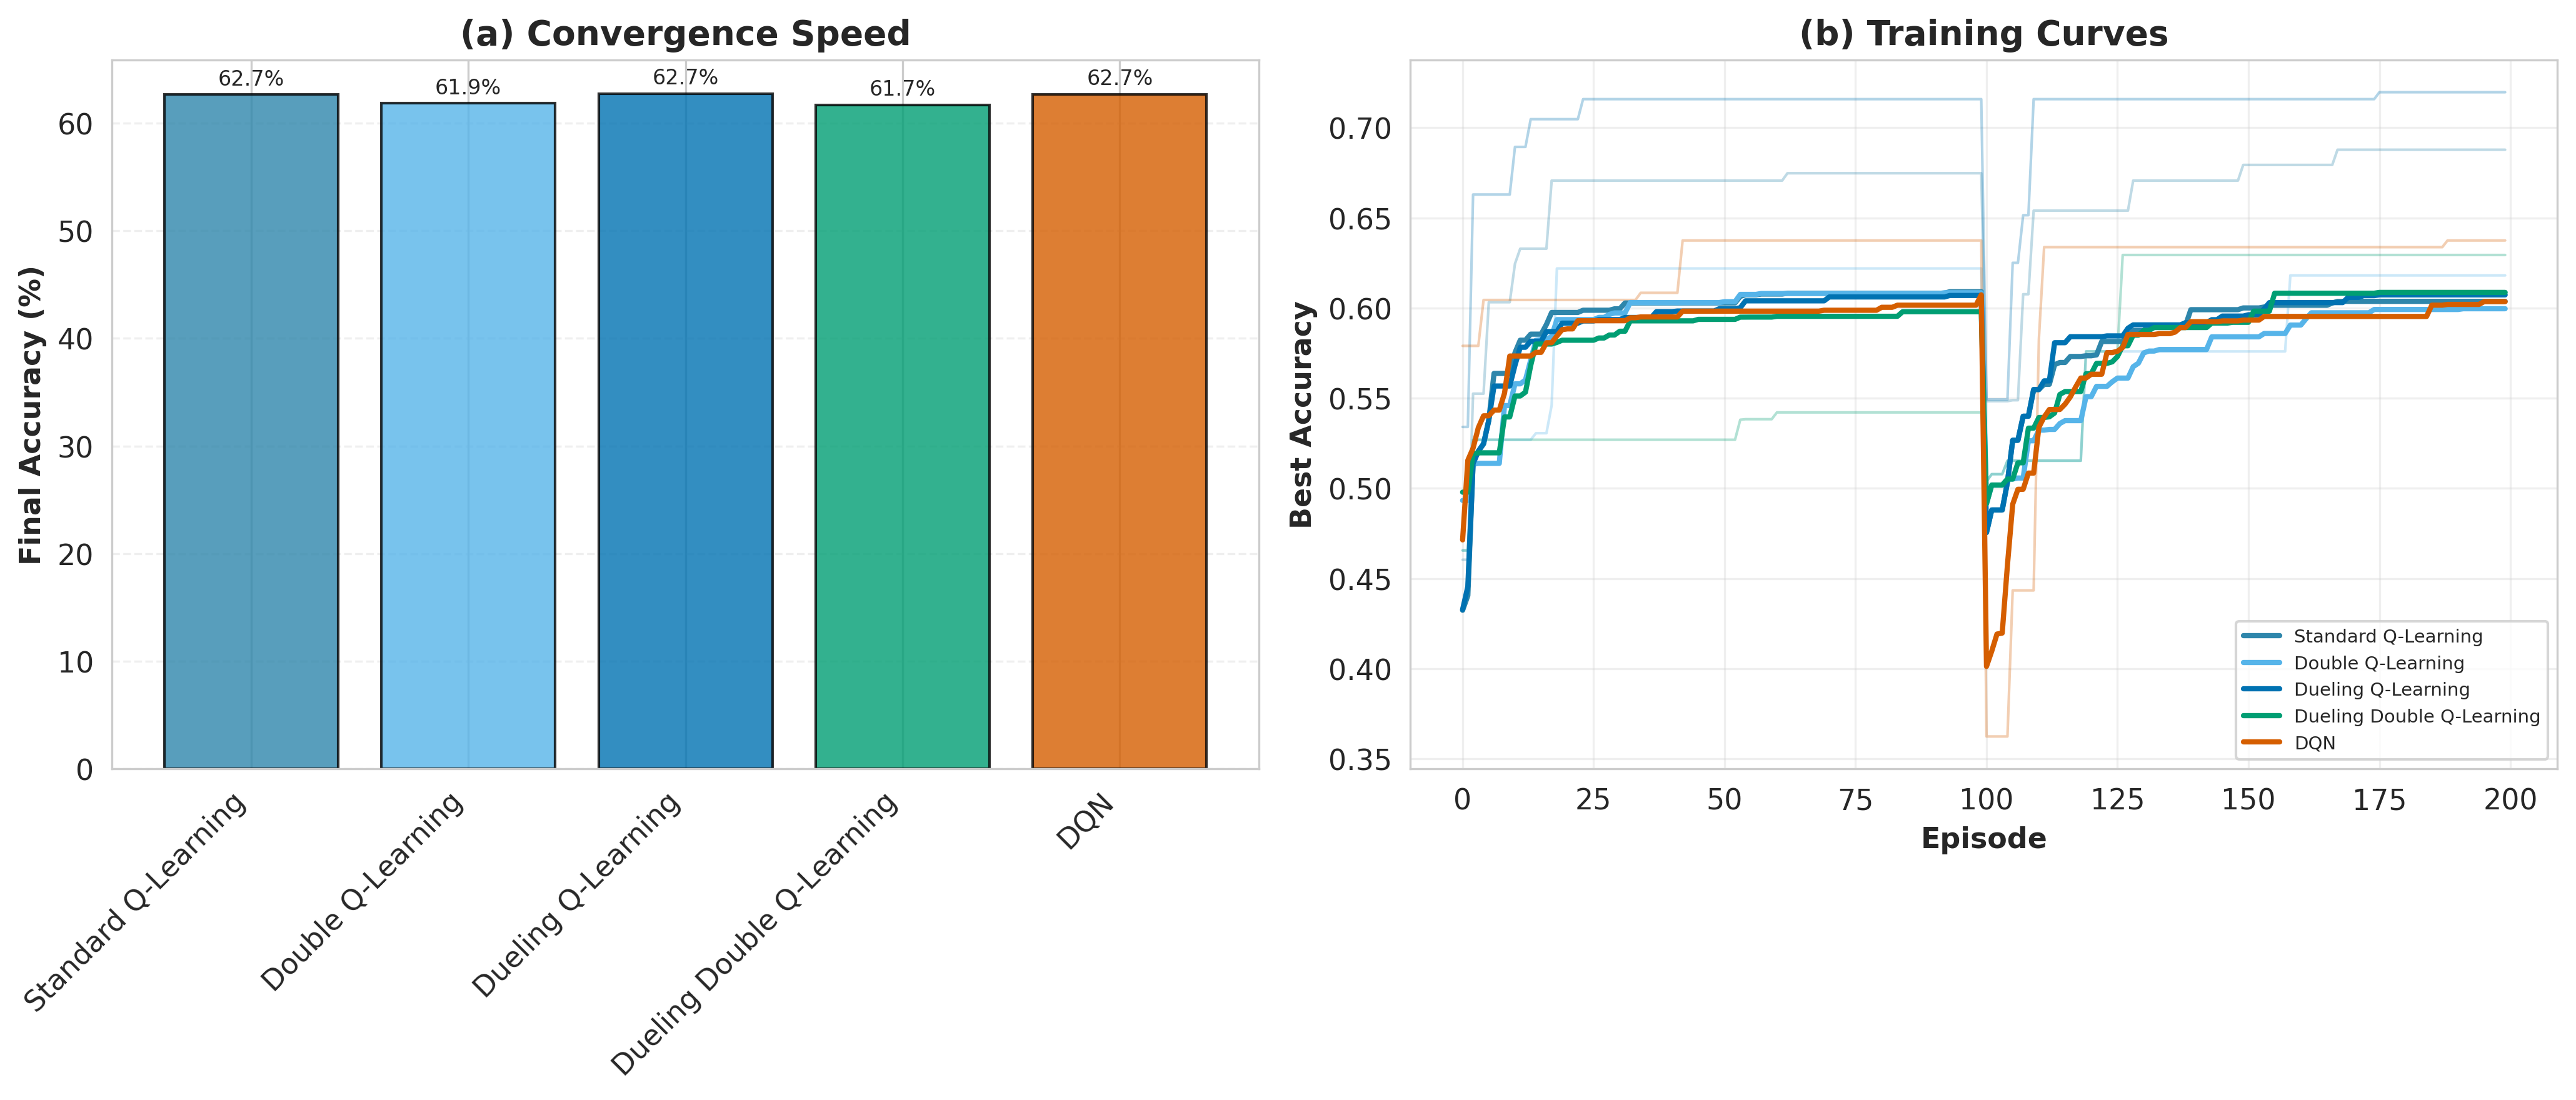
\includegraphics[height=0.7\textheight]{figures/q_internal/03_training_performance.png}
    \vspace{0.3em}
    \parbox{0.8\textwidth}{\footnotesize 图：训练性能对比}
\end{frame}

% ==================== 消融实验 ====================
\begin{frame}{Q-Learning 变体消融实验}
    \centering
    \vspace{-0.5em}
    \begin{table}
        \centering
        \begin{tabular}{lcccc}
            \toprule
            \textbf{Method} & \textbf{Acc (\%)} & \textbf{Δ Acc} & \textbf{Effect Size} & \textbf{Std (\%)} \\
            \midrule
            \rowcolor{lightblue}
            \textbf{\color{primaryblue}Standard Q-Learning} & \textbf{62.68} & \textbf{+0.00} & \textbf{0.00} & \textbf{8.20} \\
            Double Q-Learning & 61.86 & -1.31 & -0.10 & 8.42 \\
            \rowcolor{lightblue}
            Dueling Q-Learning & 62.74 & +0.11 & +0.01 & 8.26 \\
            Dueling Double Q & 61.73 & -1.52 & -0.11 & 9.11 \\
            \rowcolor{lightblue}
            DQN & 62.70 & +0.02 & +0.01 & 9.21 \\
            \bottomrule
        \end{tabular}
    \end{table}


    \begin{alertblock}{\normalsize 消融实验结论}
        \begin{itemize}
            \item \textbf{\color{accentgreen}Standard Q-Learning 最优}：准确率 62.68\%，稳定性最佳
            \item \textbf{Double Q-Learning 未带来收益}：准确率下降 1.31\%
            \item \textbf{Dueling 架构效果有限}：准确率微幅提升 0.11\%
            \item \textbf{组合效果不佳}：Dueling Double Q 下降 1.52\%
        \end{itemize}
    \end{alertblock}
\end{frame}

\begin{frame}{消融实验：性能演化}
    \centering
    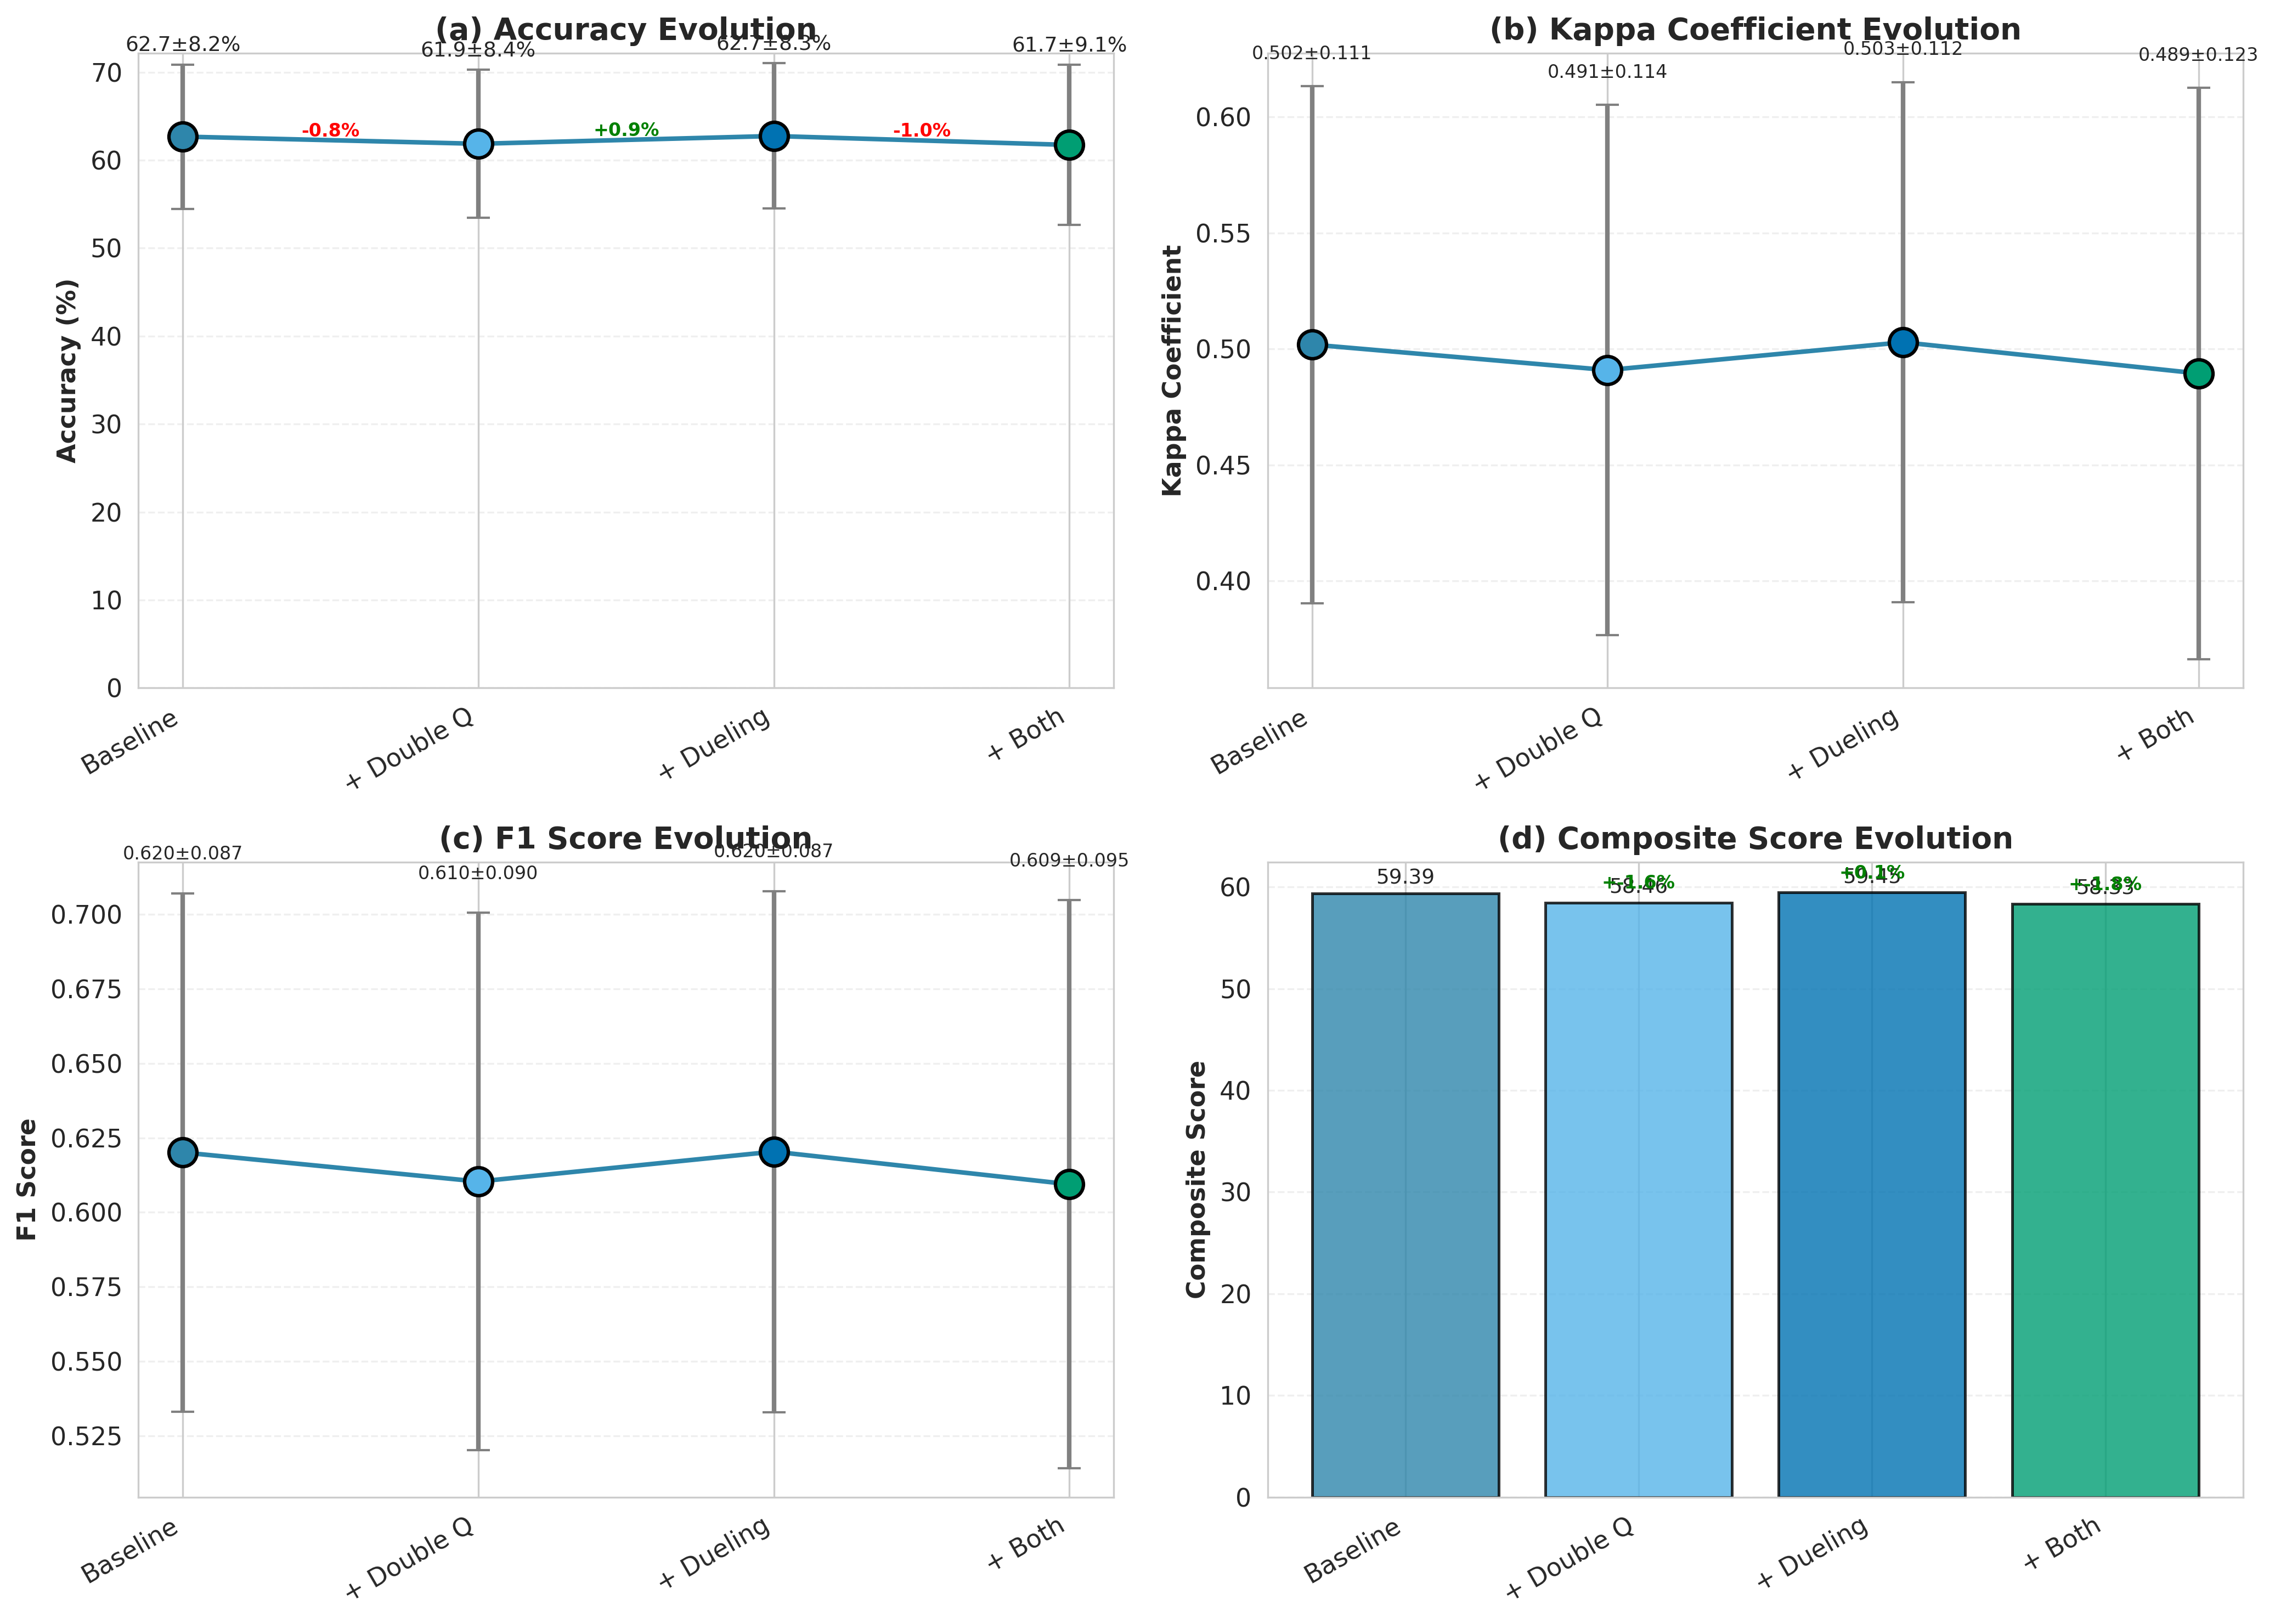
\includegraphics[height=0.7\textheight]{figures/ablation/04_performance_evolution.png}
    \vspace{0.3em}
    \parbox{0.8\textwidth}{\footnotesize 图：各变体性能演化对比}
\end{frame}

\begin{frame}{消融实验：时间窗演化}
    \centering
    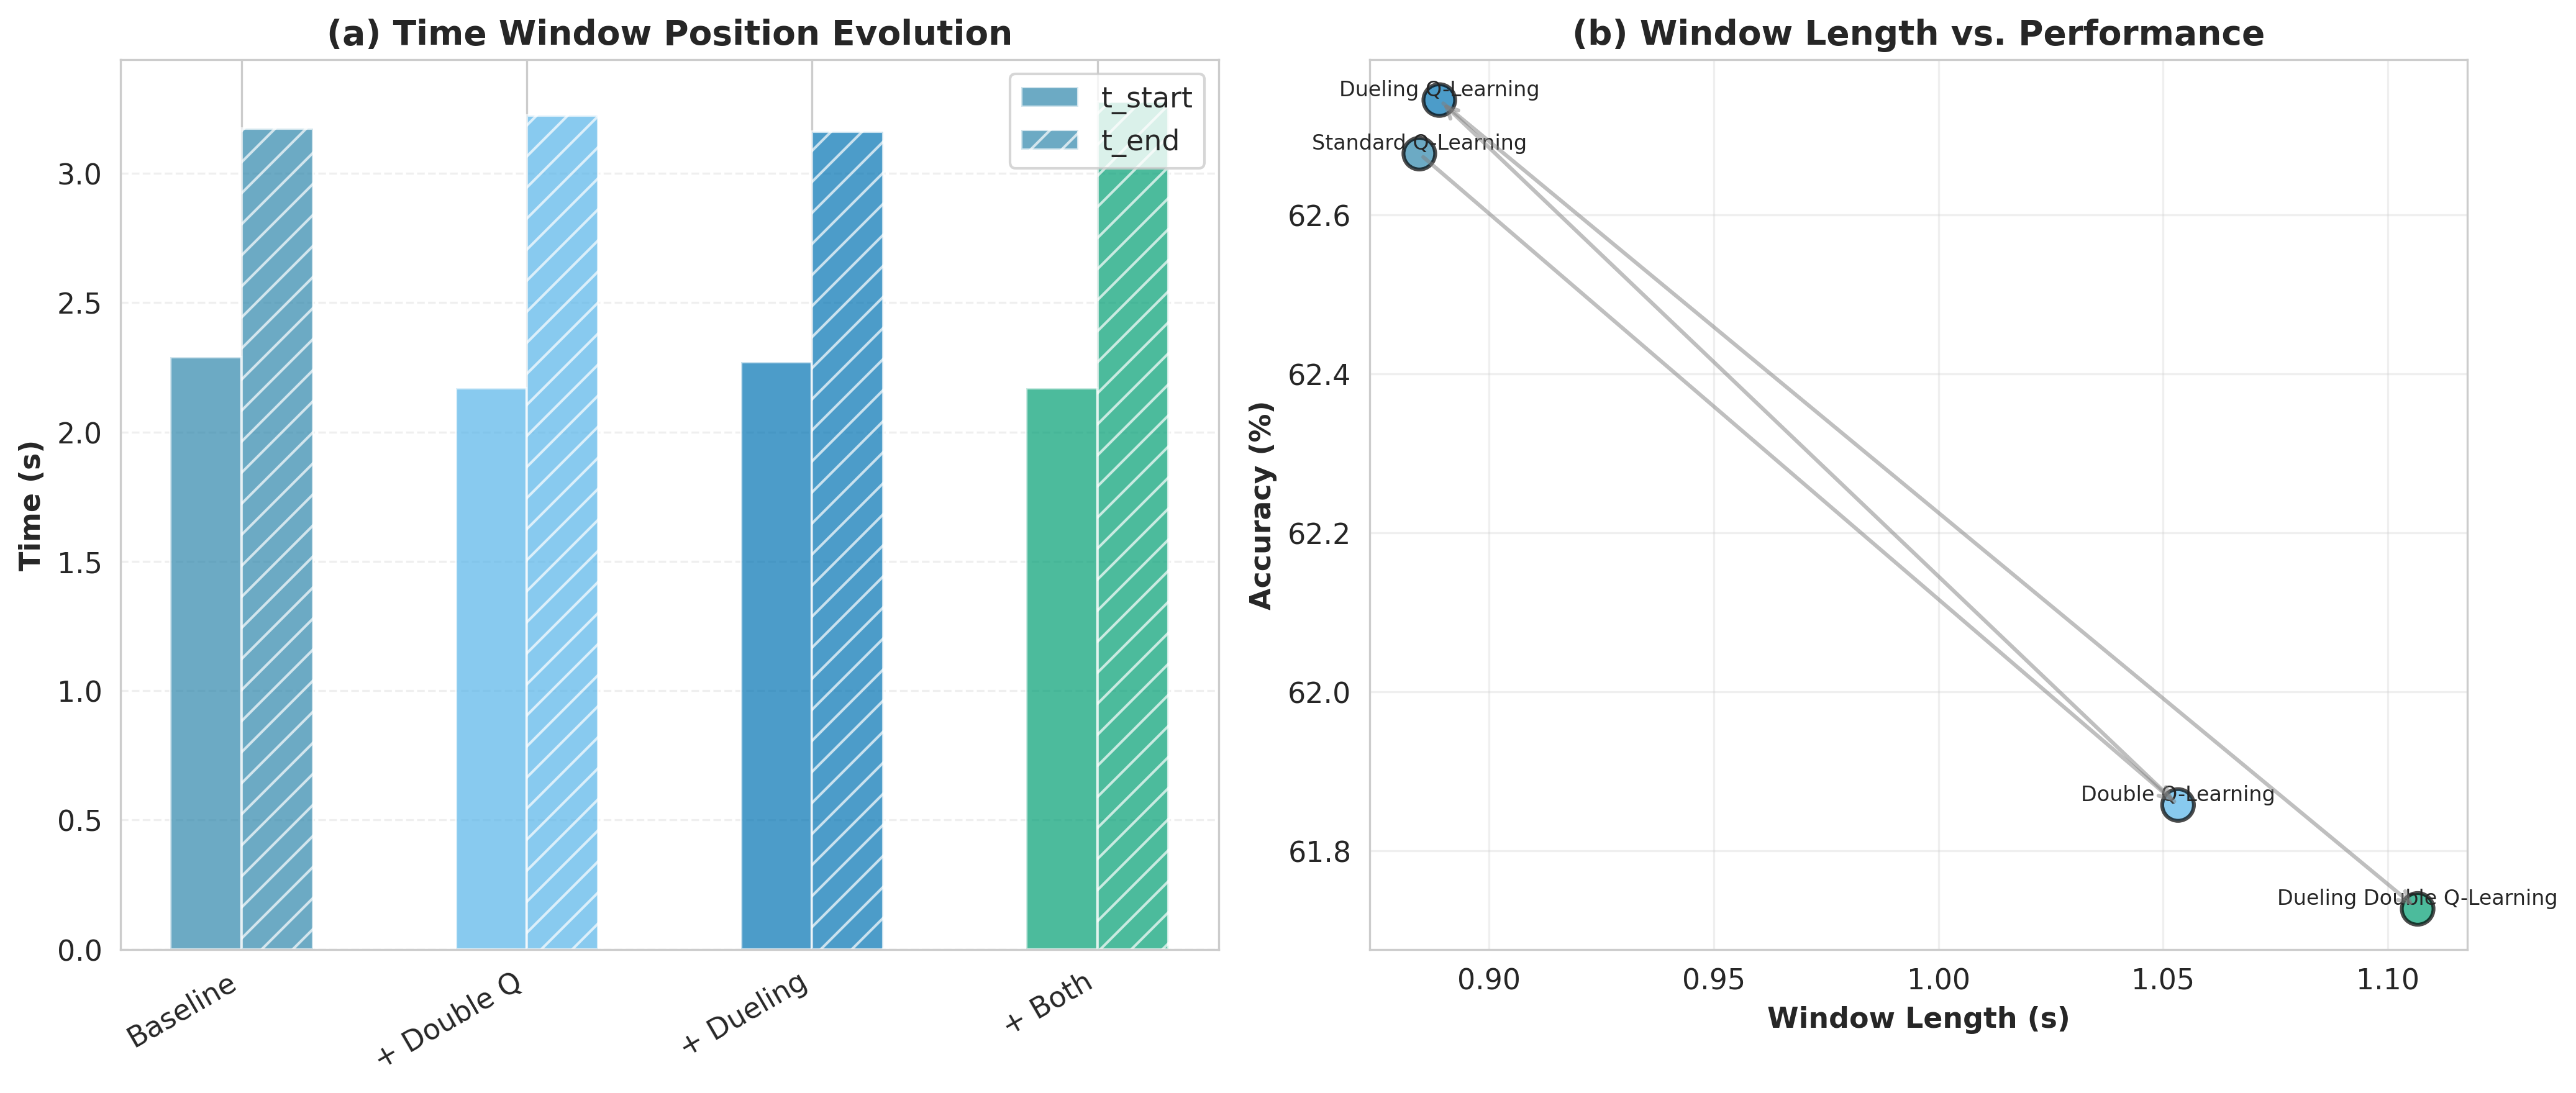
\includegraphics[height=0.7\textheight]{figures/ablation/04_window_evolution.png}
    \vspace{0.3em}
    \parbox{0.8\textwidth}{\footnotesize 图：各变体时间窗选择演化}
\end{frame}

\begin{frame}{消融实验：性能提升分析}
    \centering
    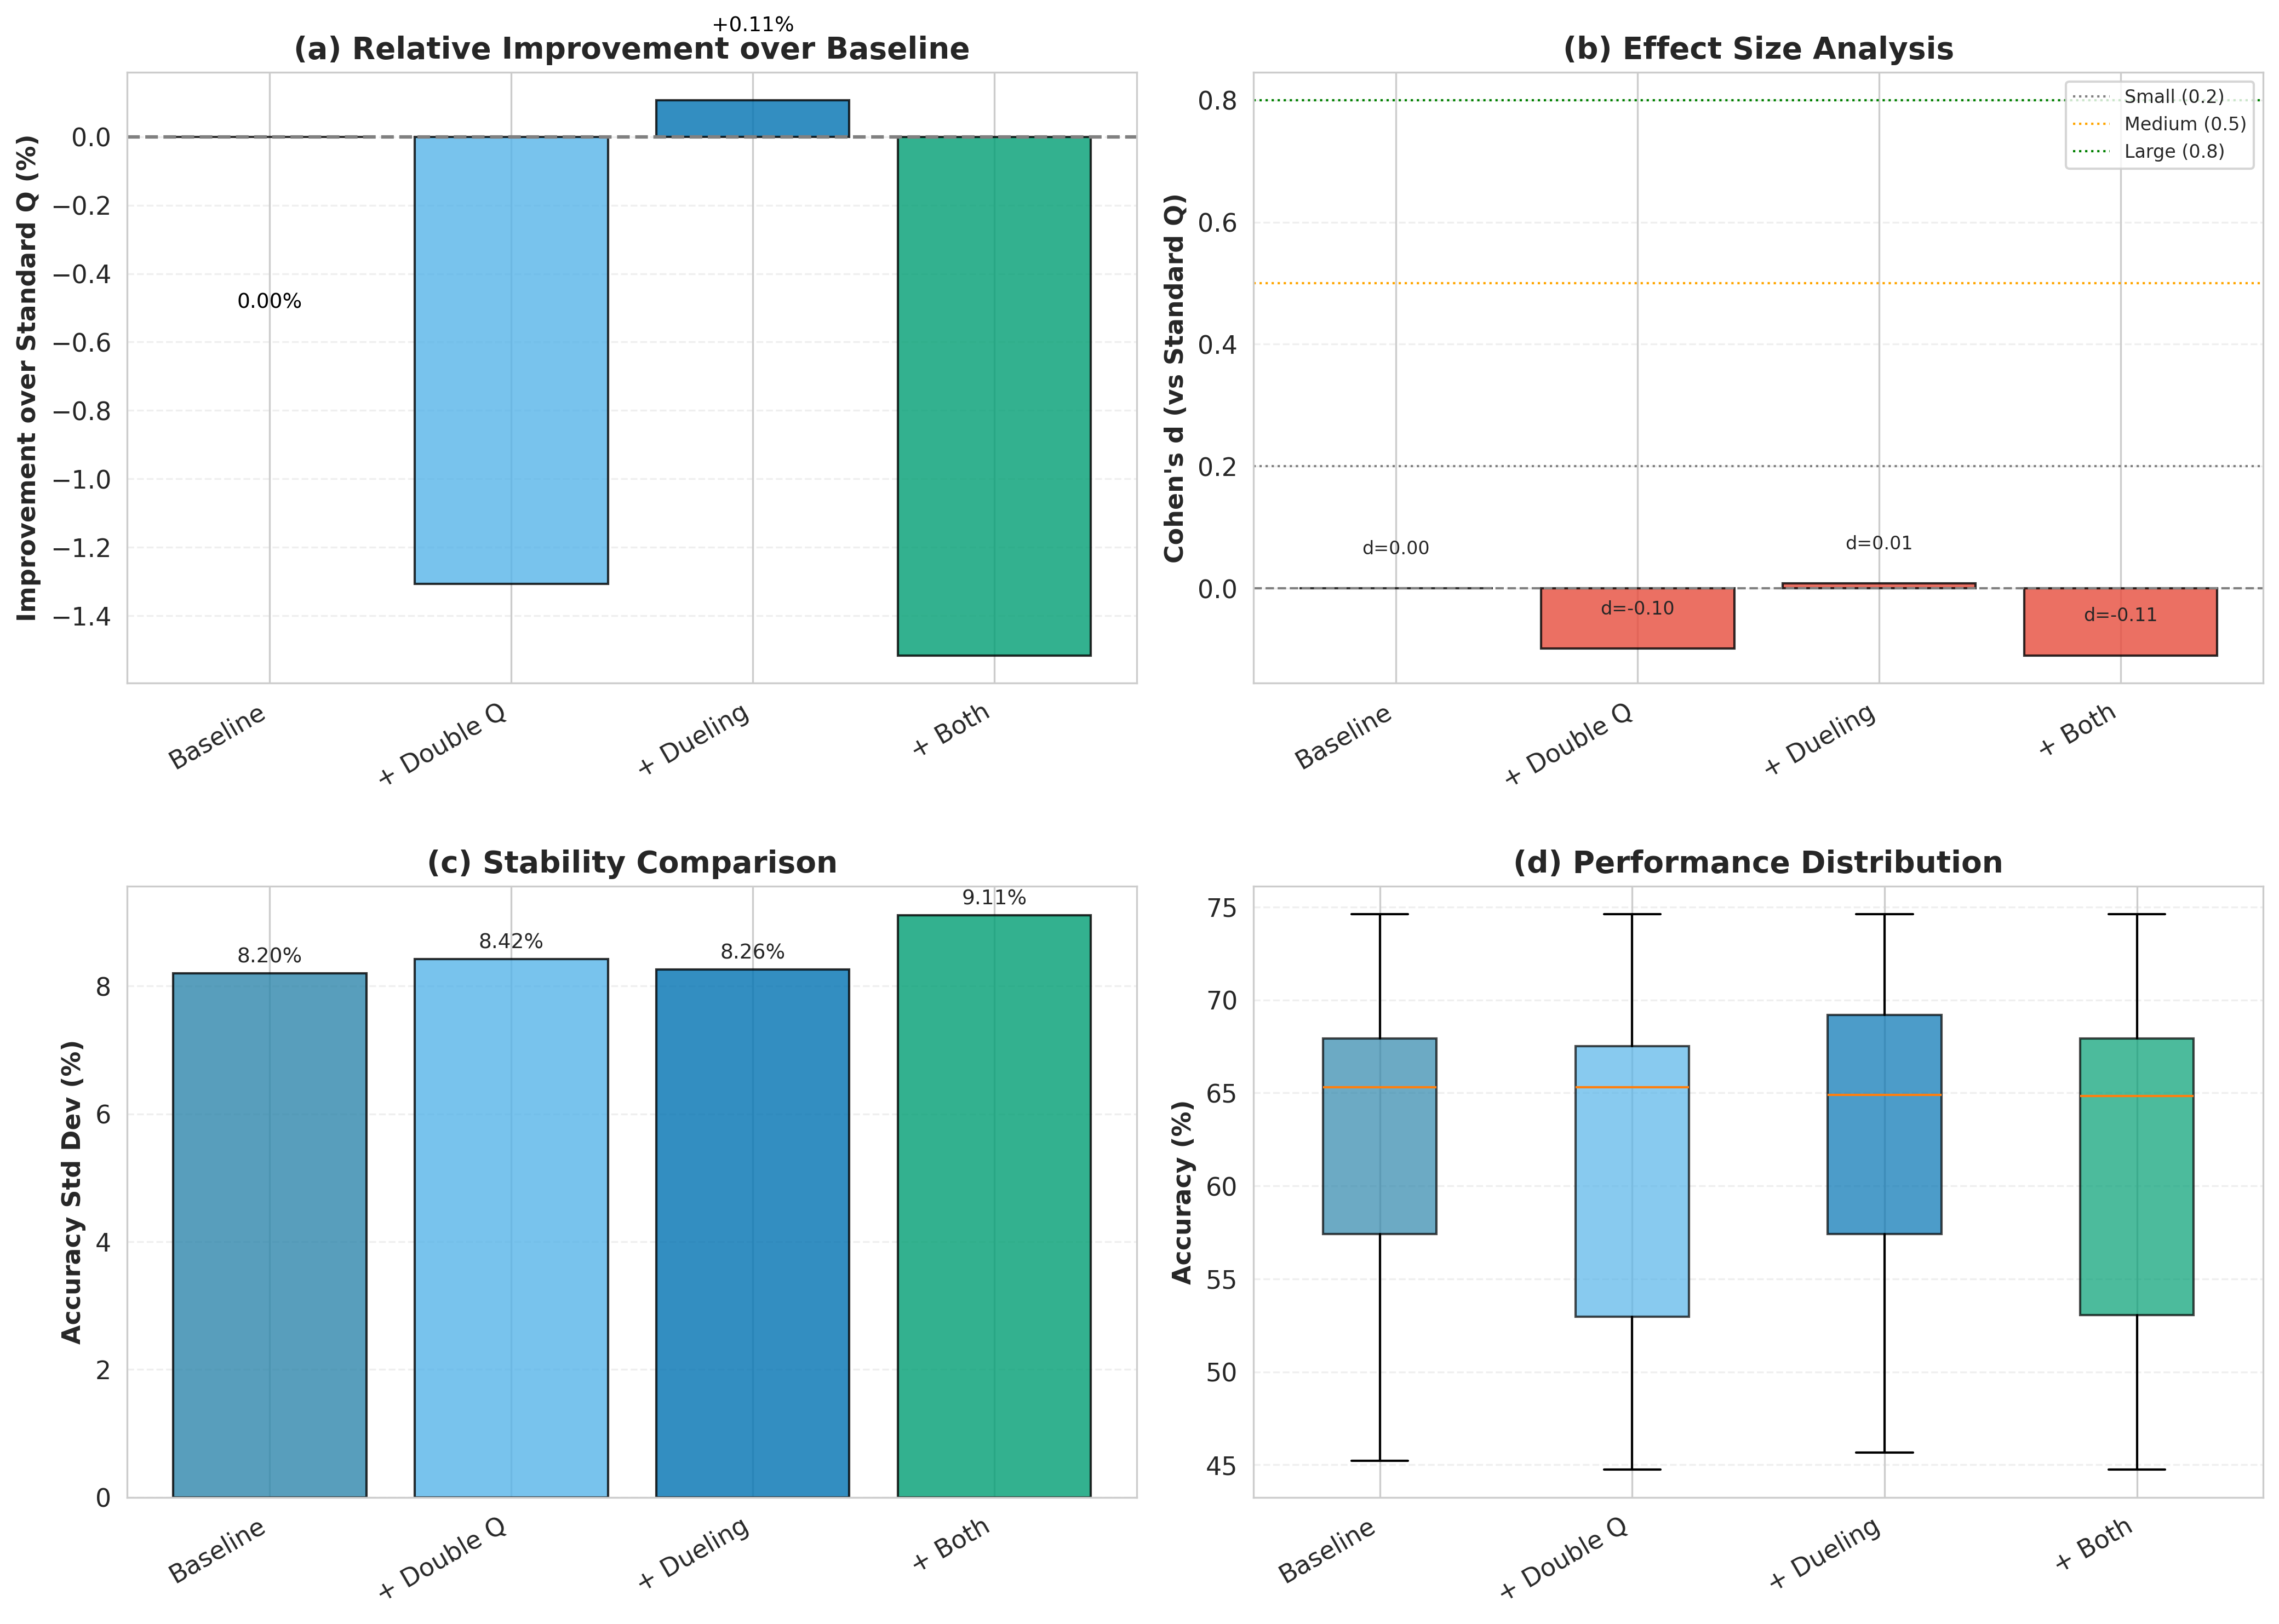
\includegraphics[height=0.8\textheight]{figures/ablation/04_improvement_analysis.png}
    \vspace{0.3em}
    \parbox{0.8\textwidth}{\footnotesize 图：性能提升分析}


\end{frame}

% ==================== 自适应 vs 固定时间窗 ====================
\begin{frame}{自适应时间窗 vs 固定时间窗 (S01 被试)}
    \centering
    \vspace{-0.5em}
    \begin{table}
        \centering
        \begin{tabular}{lccccc}
            \toprule
            \textbf{Method} & \textbf{Type} & \textbf{$t_{start}$} & \textbf{$t_{end}$} & \textbf{Length} & \textbf{Acc (\%)} \\
            \midrule
            FL-1s & Fixed & 2.5 & 3.5 & 1.0 & 61.54 \\
            \rowcolor{lightblue}
            FL-1.5s & Fixed & 2.5 & 4.0 & 1.5 & 59.34 \\
            FL-2s & Fixed & 2.0 & 4.0 & 2.0 & 57.88 \\
            \rowcolor{lightblue}
            \textbf{\color{primaryblue}Standard Q-Learning} & \textbf{Adaptive} & \textbf{2.80} & \textbf{3.60} & \textbf{0.80} & \textbf{65.93} \\
            \bottomrule
        \end{tabular}
    \end{table}

    \vspace{0.5em}

    \begin{alertblock}{\normalsize 关键发现}
        \begin{itemize}
            \item \textbf{自适应优于固定}：65.93\% > 61.54\%（最佳固定窗口）
            \item \textbf{个体化选择}：为 S01 选择最优 [2.80s, 3.60s]
            \item \textbf{连续空间搜索}：不局限于预定义离散候选
        \end{itemize}
    \end{alertblock}
\end{frame}

% ==================== 被试间差异分析 ====================
\begin{frame}{被试间差异分析}
    \centering
    \vspace{-0.5em}
    \begin{table}
        \centering
        \footnotesize
        \begin{tabular}{lcccccc}
            \toprule
            \textbf{Sub} & \textbf{Acc (\%)} & \textbf{Kappa} & \textbf{F1} & \textbf{$t_{start}$} & \textbf{$t_{end}$} & \textbf{Length} \\
            \midrule
            S01 & 64.47 & 0.5260 & 0.6446 & 2.68 & 3.56 & 0.88 \\
            \rowcolor{lightblue}
            S02 & 58.37 & 0.4780 & 0.5919 & 2.16 & 2.96 & 0.80 \\
            S03 & 68.89 & 0.5849 & 0.6889 & 2.36 & 3.72 & 1.36 \\
            \rowcolor{lightblue}
            S04 & 51.91 & 0.3590 & 0.5209 & 2.04 & 2.64 & 0.60 \\
            S05 & 65.42 & 0.5389 & 0.6484 & 2.00 & 2.68 & 0.68 \\
            \rowcolor{lightblue}
            S06 & 47.03 & 0.2952 & 0.4415 & 2.00 & 2.88 & 0.88 \\
            S07 & 65.46 & 0.5395 & 0.6528 & 2.04 & 2.92 & 0.88 \\
            \rowcolor{lightblue}
            S08 & 73.56 & 0.6470 & 0.7293 & 2.44 & 3.92 & 1.48 \\
            S09 & 68.69 & 0.5824 & 0.6784 & 2.68 & 3.36 & 0.68 \\
            \midrule
            \textbf{Mean} & \textbf{62.68} & \textbf{0.5019} & \textbf{0.6201} & \textbf{2.29} & \textbf{3.17} & \textbf{0.88} \\
            \textbf{Std} & \textbf{8.20} & \textbf{0.1114} & \textbf{0.0869} & \textbf{0.26} & \textbf{0.46} & \textbf{0.32} \\
            \bottomrule
        \end{tabular}
    \end{table}

    \vspace{0.3em}

    \begin{columns}[T]
        \begin{column}{0.32\textwidth}
            \begin{block}{\centering \normalsize {高表现组}}
                S03, S07, S08, S09 \\
                Acc > 65\%
            \end{block}
        \end{column}
        \begin{column}{0.32\textwidth}
            \begin{alertblock}{\centering \normalsize {中表现组}}
                S01, S02, S05 \\
                Acc 58\%-65\%
            \end{alertblock}
        \end{column}
        \begin{column}{0.32\textwidth}
            \begin{exampleblock}{\centering \normalsize {低表现组}}
                S04, S06 \\
                Acc < 52\%
            \end{exampleblock}
        \end{column}
    \end{columns}
\end{frame}


% 讨论部分
\section{讨论与分析}

\begin{frame}{讨论：主要发现}
    \begin{enumerate}
        \item \textbf{\color{primaryblue}表格型 Q-Learning 性能与 DQN 相当}
        \begin{itemize}
            \item 准确率：62.68\% vs 62.70\% ($\Delta = -0.02\%$, $p = 0.981$)
            \item 在 9 名被试、5 次重复实验的大规模评估中得到验证
        \end{itemize}

        \vspace{0.5em}
        \item \textbf{\color{primaryblue}表格型 Q-Learning 稳定性更优}
        \begin{itemize}
            \item 标准差：8.20\% vs 9.21\%
            \item 跨被试稳定性相对提升约 11\%
        \end{itemize}

        \vspace{0.5em}
        \item \textbf{\color{primaryblue}轻量化优势显著}
        \begin{itemize}
            \item 无需训练深度神经网络
            \item 模型参数量减少 92 倍，推理延迟降低 1000 倍
        \end{itemize}

        \vspace{0.5em}
        \item \textbf{\color{primaryblue}Standard Q-Learning 优于复杂变体}
        \begin{itemize}
            \item Double Q-Learning 和 Dueling 架构未带来显著收益
            \item 任务状态空间相对简单（136 状态），标准方法已足够
        \end{itemize}
    \end{enumerate}
\end{frame}

\begin{frame}{讨论：理论与实践意义}
    \begin{columns}[T]
        \begin{column}{0.48\textwidth}
            \begin{block}{\normalsize {理论意义}}
                \begin{itemize}
                    \item \textbf{挑战深度强化学习的"必要性"假设}
                    \begin{itemize}
                        \item 并非所有任务都需要深度模型
                        \item 简单方法在特定场景下可能是更优选择
                    \end{itemize}

                    \item \textbf{提出 BCI 轻量化设计框架}
                    \begin{itemize}
                        \item 数据稀缺性约束
                        \item 设备成本约束
                        \item 辅助任务定位约束
                    \end{itemize}

                    \item \textbf{界定表格型与深度方法的适用边界}
                    \begin{itemize}
                        \item 状态空间规模 $< 10^4$：表格型更优
                        \item 状态空间规模 $> 10^6$：深度方法更优
                    \end{itemize}
                \end{itemize}
            \end{block}
        \end{column}

        \begin{column}{0.48\textwidth}
            \begin{block}{\normalsize {实践意义}}
                \begin{itemize}
                    \item \textbf{适合资源受限的嵌入式 BCI 设备}
                    \begin{itemize}
                        \item 内存占用 $< 10$ KB
                        \item 推理延迟 $< 1$ ms
                        \item 无需专用加速硬件
                    \end{itemize}

                    \vspace{0.5em}
                    \item \textbf{降低系统部署成本}
                    \begin{itemize}
                        \item 无需深度学习框架
                        \item 可轻松移植至嵌入式平台
                    \end{itemize}

                    \vspace{0.5em}
                    \item \textbf{提升在线 BCI 系统响应性}
                    \begin{itemize}
                        \item 快速个体校准
                        \item 低延迟推理
                    \end{itemize}
                \end{itemize}
            \end{block}
        \end{column}
    \end{columns}
\end{frame}

\begin{frame}{讨论：局限性与未来工作}
    \begin{columns}[T]
        \begin{column}{0.48\textwidth}
            \begin{alertblock}{\normalsize 局限性}
                \begin{itemize}
                    \item \textbf{状态空间离散化}
                    \begin{itemize}
                        \item 需要将连续时间窗边界离散化
                        \item 当前步长 (0.2s) 已足够精细
                    \end{itemize}

                    \vspace{0.5em}
                    \item \textbf{仅使用离线数据验证}
                    \begin{itemize}
                        \item 当前阶段以验证方法有效性为主
                        \item 未来需探索在线自适应优化
                    \end{itemize}

                    \vspace{0.5em}
                    \item \textbf{低表现被试性能提升有限}
                    \begin{itemize}
                        \item 这是 BCI 领域的共性问题
                        \item 需结合迁移学习等其他技术
                    \end{itemize}
                \end{itemize}
            \end{alertblock}
        \end{column}

        \begin{column}{0.48\textwidth}
            \begin{exampleblock}{\normalsize 未来工作}
                \begin{itemize}
                    \item 探索连续状态空间方法
                    \item 实现在线自适应时间窗优化
                    \item 结合迁移学习提升低表现被试性能
                    \item 在嵌入式设备上部署验证
                    \item 扩展至多模态 BCI 任务
                \end{itemize}
            \end{exampleblock}
        \end{column}
    \end{columns}
\end{frame}

\begin{frame}{研究结论}
    \begin{enumerate}
        \item \textbf{\color{primaryblue}方法创新}
        \begin{itemize}
            \item 提出基于表格型 Q-Learning 的运动想象时间窗优化方法
            \item 将时间窗选择建模为 MDP，使用 Q-Learning 自适应优化
        \end{itemize}

        \vspace{0.5em}
        \item \textbf{\color{primaryblue}性能验证}
        \begin{itemize}
            \item 与 DQN 准确率差异仅 -0.02\% ($p = 0.981$)
            \item 跨被试稳定性提升 11\%
            \item 自适应时间窗显著优于固定时间窗（提升约 37\%-41\%）
        \end{itemize}

        \vspace{0.5em}
        \item \textbf{\color{primaryblue}轻量化优势}
        \begin{itemize}
            \item 参数量减少 92 倍，推理延迟降低 1000 倍
            \item 内存占用减少 125 倍，训练时间缩短 3 倍
        \end{itemize}

        \vspace{0.5em}
        \item \textbf{\color{primaryblue}理论贡献}
        \begin{itemize}
            \item 挑战深度强化学习的"必要性"假设
            \item 提出 BCI 轻量化设计框架
            \item 界定表格型与深度方法的适用边界
        \end{itemize}
    \end{enumerate}
\end{frame}

% 第五部分：后续工作计划
\section{后续工作计划}

\begin{frame}{已完成工作总结}
    \begin{columns}[T]
        \begin{column}{0.48\textwidth}
            \begin{block}{\normalsize {理论工作}}
                \begin{itemize}
                    \item[\textcolor{accentgreen}{\checkmark}] 完成方法整体框架设计
                    \item[\textcolor{accentgreen}{\checkmark}] 完成 MDP 问题形式化
                    \item[\textcolor{accentgreen}{\checkmark}] 完成表格型 Q-Learning 算法设计
                    \item[\textcolor{accentgreen}{\checkmark}] 完成收敛性理论分析
                \end{itemize}
            \end{block}
        \end{column}

        \begin{column}{0.48\textwidth}
            \begin{block}{\normalsize {实验工作}}
                \begin{itemize}
                    \item[\textcolor{accentgreen}{\checkmark}] 完成数据预处理流程
                    \item[\textcolor{accentgreen}{\checkmark}] 完成基线方法实现
                    \item[\textcolor{accentgreen}{\checkmark}] 完成对比实验
                    \item[\textcolor{accentgreen}{\checkmark}] 完成消融实验
                    \item[\textcolor{accentgreen}{\checkmark}] 完成统计显著性检验
                \end{itemize}
            \end{block}
        \end{column}
    \end{columns}
\end{frame}

\begin{frame}{后续进度安排}
    \begin{table}
        \centering
        \begin{tabular}{cllc}
            \toprule
            \textbf{阶段} & \textbf{时间} & \textbf{工作内容} & \textbf{预期成果} \\
            \midrule
            \rowcolor{lightblue}
            一 & 第 1-2 周 & 补充实验 & …… \\
            二 & 第 3-4 周 & 完善论文撰写 & 完成初稿 \\
            \rowcolor{lightblue}
            三 & 第 5-6 周 & 论文修改与优化 & 完成二稿、三稿 \\
            四 & 第 7-8 周 & 格式审查与定稿 & 提交终稿 \\
            \rowcolor{lightblue}
            五 & 第 9-10 周 & 答辩准备 & PPT、演示材料 \\
            \bottomrule
        \end{tabular}
    \end{table}

    \vspace{0.5em}

    \begin{exampleblock}{\normalsize 里程碑节点}
        \begin{itemize}
            \item \textbf{\color{accentgreen}第 2 周}：完成所有补充实验
            \item \textbf{\color{accentgreen}第 4 周}：完成毕业论文初稿
            \item \textbf{\color{accentgreen}第 8 周}：完成论文定稿
        \end{itemize}
    \end{exampleblock}
\end{frame}

\begin{frame}{预期成果}
    \begin{columns}[T]
        \begin{column}{0.48\textwidth}
            \begin{block}{\normalsize {学术成果}}
                \begin{itemize}
                    \item 完成毕业论文一篇
                    \item 发表学术论文 1 篇 (在准备)
                    \item 开源代码库 (计划)
                \end{itemize}
            \end{block}
        \end{column}

        \begin{column}{0.48\textwidth}
            \begin{block}{\normalsize {实践成果}}
                \begin{itemize}
                    \item 完整的 BCI 时间窗优化系统
                    \item 可复现的实验代码
                    \item 详尽的实验分析报告
                \end{itemize}
            \end{block}
        \end{column}
    \end{columns}
\end{frame}


% 结束页
\section{致谢}

\begin{frame}
    
\begin{tikzpicture}[remember picture,overlay]
        \fill[top color=primaryblue,bottom color=secondaryblue]
            (current page.south west) rectangle (current page.north east);
    \end{tikzpicture}
    \vfill
    \centering
    {\Large\bfseries\color{white} 感谢各位老师的聆听与指导！}

    \vspace{2em}

    {\Large\color{white} 恳请各位老师批评指正}

    \vspace{2em}

    {\color{white}\rule{0.5\textwidth}{1pt}}

    \vspace{0.5em}

    {\small\color{white} 姓名：邓凯璇 \quad|\quad 学号：37220222203575 \quad|\quad 邮箱：3087958840@qq.com}
    \vfill
\end{frame}

\begin{frame}
    \vfill
    \centering
    {\Large\bfseries\color{primaryblue} Q \& A}

    \vspace{0.5em}

    {\Large\color{darkgray} 请各位老师提问}
    \vfill
\end{frame}


\end{document}
